\documentclass[ngerman,12pt,listof=totoc, bibliography=totoc ]{scrartcl}

% Preamble und Konfiguration laden
%-------------------------------------------------------
%-----------------------------------------------------------------------------------------------------------------------
%Abkürzungsverzeichnis
\usepackage[printonlyused]{acronym}

%Sprache festlegen auf Deutsch
\usepackage[ngerman]{babel} 

%Quellenverzeichnis
\usepackage[natbib=true, backend=biber, style=authoryear, dashed=false]{biblatex}
\addbibresource{content/bib/bibliography.bib}

%Schriftart
\usepackage{carlito}
\setmainfont{carlito}

%Fortgeschrittene Funktionen für Zitate 
\usepackage{csquotes}

%Positionierung von Tabellen und Abbildungen
\usepackage{float}

%OpenType fonts können geladen werden
\usepackage{fontspec}

%Seitenränder einstellen
\usepackage[left=3.0cm, right=3.0cm, head=2.5cm, bottom=3cm]{geometry}

%Abbildungen
\usepackage{graphicx}  
\graphicspath{{content/images/}}

%Verweise
\usepackage[hidelinks]{hyperref}
\usepackage{cleveref}   %cleveref muss nach hyperref geladen werden

%Header / Footer
\usepackage[headsepline,footsepline,plainfootsepline]{scrlayer-scrpage}
\renewcommand*{\sectionmarkformat}{} %lässt die Nummerierungszahl der Section aus dem Header verschwinden
\clearpairofpagestyles
\ohead{\headmark}
\automark{section}
\ofoot[\pagemark]{\pagemark}
\cfoot[\thesistitel]{\thesistitel}

%Zeilenabstand einstellen
\usepackage[onehalfspacing]{setspace}

%Bilder, Tabellen etc. nebeneinander platzieren
\usepackage{subcaption}

%Für Notizen
\usepackage[colorinlistoftodos,prependcaption]{todonotes}

% Wird gebraucht um Fehlermeldung wegzubekommen
\setlength {\marginparwidth }{2cm} 

%TODOS
\newcommand{\comingSoon}[1]{\todo[inline,linecolor=red,backgroundcolor=red!40, bordercolor=black]{#1}}
\newcommand{\change}[1]{\todo[linecolor=blue, backgroundcolor=blue!40, bordercolor=black]{#1}}
\newcommand{\info}[1]{\todo[shadow, noline,linecolor=green, backgroundcolor=green!40, bordercolor=black]{#1}}
\newcommand{\improvement}[1]{\todo[linecolor=violet,backgroundcolor=violet!40,bordercolor=black]{#1}}

%Farben
\usepackage{xcolor}

%-----------------------------------------------------------------------------------------------------------------------
%Counter um die Seiten zu zählen, für römische Zahlen
\newcounter{seitenanzahl}
%Inhaltsverzeichnis ins Inhaltsverzeichnis
\setuptoc{toc}{totoc}
%-----------------------------------------------------------------------------------------------------------------------


%Namen des Autors
\newcommand{\thesisauthor}{Ghaith Dmirieh}

%Titel der Arbeit
\newcommand{\thesistitel}{Codereview-System}

%Genaue Bezeichnung der Arbeit
\newcommand{\thesistyp}{Projektarbeit 1}

%Abgabedatum der Arbeit
\newcommand{\abgabedatum}{XX.XX.2020}

%Kursname
\newcommand{\kurs}{TIF-19A}

%Studiengang
\newcommand{\studiengang}{Informatik}

%Abschluss
%\newcommand{\abschluss}{Bachelor of Science}

%Name des Unternehmens
\newcommand{\unternehmen}{Mimot GmbH}

%Name des Betreuers im Unternehmen
\newcommand{\unternehmensbetreuer}{Björn Schäpers}

%Standort des Unternehmens
\newcommand{\arbeitsort}{Lörrach}

%Name des DHBW-Betreuers
\newcommand{\dhbwbetreuer}{Kein Betreuer}

%Datum für die ehrenwörtliche Erklärung
\newcommand{\datumerklaerung}{XX.XX.2020}

%Ort der ehrenwörtlichen Erklärung
\newcommand{\orterklaerung}{Lörrach}

%Datum der Freigabe durch das Unternehmen
\newcommand{\datumfreigabe}{XX.XX.2020}

%Ort der Freigabe 
\newcommand{\ortfreigabe}{Lörrach}

%Datum der Unterschrift des Autors beim Sperrvermerk
\newcommand{\sperrvermerkdatumauthor}{XX.XX.2020}

%Datum der Unterschrift des Unternehmens beim Sperrvermerk
\newcommand{\sperrvermerkdatumunternehmen}{XX.XX.2020}

%Adresse des Unternehmens
\newcommand{\unternehmensadresse}{Berner Weg 11, 79539 Lörrach}

%Email des Unternehmens
\newcommand{\unternehmsemail}{ghaith.dmirieh@mimot.com}

%Telefonnummer des Unternehmens
\newcommand{\unternehmenstel}{+49 (0) 76 21 - 95 78 0}

%Variable ob es sich um eine Studienarbeit handelt
\newif\ifseminararbeit  %Deklaration
\seminararbeitfalse     %Zuweisung des Wertes true

%Variable ob es einen Sperrvermerk gibt
\newif\ifsperrvermerk   %Deklaration
\sperrvermerktrue       %Zuweisung des Wertes true

%Variable ob es einen DHBW-Betreuer gibt
\newif\ifdhbwbetreuer   %Deklaration
\dhbwbetreuerfalse      %Zuweisung des Wertes false

%-------------------------------------------------------

\begin{document}

\author{\thesisauthor}
\title{\thesistitle}
\date{\abgabedatum}
\pagestyle{plain.scrheadings}
\pagenumbering{Roman}

\thispagestyle{empty}

\vspace*{-2.5cm}

\ifseminararbeit
\else

\includegraphics[width=6cm]{mimot-Logo}
\fi
\hfill

\includegraphics[width=6cm]{logo-dhbw}
\vspace*{3cm}

\begin{center}
{\LARGE \thesistitel} \\
\vspace{0.5cm}

\ifsperrvermerk 
\textcolor{red}{\large SPERRVERMERK\\}
\else
\vspace{2cm}
\fi

\vspace{1cm}

\textbf{\large \thesistyp}\\

%\vspace{2cm}
%für die Prüfung zum \\ 
%\abschluss \\

\vspace{2cm} 
des Studiengangs \studiengang \\
an der \\
Dualen Hochschule Baden-Württemberg Lörrach \\

\vspace{1cm}
\thesisauthor \\
\abgabedatum
\vfill

\begin{tabular}{l l}
Kurs & \kurs \\
Ausbildungsunternehmen & \unternehmen \\

\ifseminararbeit
\else
Unternehmensbetreuer & \unternehmensbetreuer \\
\fi

\ifdhbwbetreuer
Wissenschaftlicher Betreuer & \dhbwbetreuer \\
\fi

\end{tabular}
\end{center}
\addsec{Ehrenwörtliche Erklärung}
\noindent Ich versichere hiermit, dass ich meine \thesistyp{} mit dem Thema:
\begin{center}
\textbf{ \thesistitel}
\end{center}

\noindent selbstständig verfasst und keine anderen als die angegebenen Quellen und Hilfsmittel benutzt habe. Ich versichere zudem, dass die 				  eingereichte elektronische Fassung mit der gedruckten Fassung übereinstimmt.

\vspace*{1cm}
\noindent \orterklaerung, \datumerklaerung{} \\
\vspace*{1.5cm} \\
\noindent\rule{8cm}{0.5pt}\\
\thesisauthor
\vfill*

\addsec{Hinweise zum Umfang der Arbeit}

\noindent Der Textteil der vorliegenden Arbeit - beginnend mit der Einleitung bis ausschließlich Quellenverzeichnis - umfasst \pageref{seitenreinschrifft} Seiten.




\ifseminararbeit
\else
\addsec{Freigabe der Arbeit}
\noindent Die vorliegende Arbeit wurde durch das Ausbildungsunternehmen 
\unternehmen{}, inhaltlich geprüft und zur Vorlage an der DHBW Lörrach, Studiengang \kurs, freigegeben.

\vspace*{4cm}
\begin{center}
	\begin{tabular}[h]{cc}
		\noindent\rule{7cm}{0.5pt} & \noindent\rule{7cm}{0.5pt} \\
		\noindent\ortfreigabe, \datumfreigabe & \unternehmensbetreuer
 	\end{tabular}
\end{center}

\fi

\ifsperrvermerk 
\addsec{Sperrvermerk}
Der Inhalt dieser Arbeit darf weder als Ganzes noch in Auszügen Personen außerhalb des Prüfungsprozesses und des Evaluationsverfahrens zugänglich gemacht werden, sofern keine anders lautende Genehmigung der Ausbildungsstätte vorliegt.
\vspace{4cm}
\begin{center}
 \begin{tabular}[h]{cc}
   \noindent\rule{7cm}{0.5pt} & \noindent\rule{7cm}{0.5pt} \\
   \noindent\sperrvermerkdatumauthor, \thesisauthor & \sperrvermerkdatumunternehmen, \unternehmensbetreuer
 \end{tabular}
\end{center}
\vspace{2cm}
\textbf{Kontakt:} \\
\unternehmen \\
\unternehmensadresse \\
\unternehmsemail \\
\unternehmenstel 

\fi

\addsec{Kurzfassung}

Codereview bedeutet, dass andere Teammitglieder die Quelltext-Änderungen vom Autor kritisieren. Dieser Prozess ist eine gute Übung sowohl in Open Source als auch in privaten Softwarebereichen. Der heutige Codereview ist weniger formal und leichter als die Codereview, die in den 70er und 80er Jahren durchgeführt und untersucht wurden. Die Studien zeigten, dass zwar die Fehlererkennung das Hauptziel ist, jedoch traten weniger Fehler als erwartet auf. Stattdessen gab es zusätzliche Vorteile wie Wissenstransfer, Teambewusstsein und die Schaffung alternativer Problemlösungen. Es Wurde festgestellt, dass das Verständnis von Code und Änderungen der Schlüsselaspekt vom Codereview \cite{bacchelli2013expectations}.
\tableofcontents

\addsec{Abkürzungsverzeichnis}

\begin{acronym}[VCS] % Das Paket kann nicht automatisch sortieren
\acro{CD}{Continuous Delivery/Continuous Deployment}
\acro{CI}{Continuous Integration}
\acro{CRS}{Codereview-System}
\acrodefplural{CRS}[CRSe]{Codereview-Systeme}
\acro{SVN}{Apache Subversion}
\acro{CVN}{Concurrent Versions System}
\acro{VCS}{Version Control System}
\acrodefplural{VCS}[VCSe]{Version Control Systeme}
\acro{IDE}{Integrated development environment}
\end{acronym}

\clearpage
\listoffigures
\clearpage
\listoftables
\clearpage
\setcounter{seitenanzahl}{\value{page}}
\pagenumbering{arabic}
\pagestyle{scrheadings}

%Hier kommen die eigentlichen Kapitel
%-----------------------------------------------------------
\section{Einleitung}

\section{Grundlagen}
\label{sec:Grundlagen}

\subsection{Definition}
\label{subsec:Definition}

\begin{description}
	\item [Codereview:]
		Unter Codereview Versteht man, eine manuelle Überprüfung des Quellcodes durch andere Entwickler als den Autor. Es gilt als wertvolles Werkzeug zur Reduzierung von 							Softwarefehlern und zur Verbesserung der Qualität von Softwareprojekten \cite{bacchelli2013expectations}.

	\item [VCS:]
		"`Versionskontrollsysteme sind Softwaretools, mit deren Hilfe Softwareteams Quellcodeänderungen verwalten können. Die Versionskontrollsoftware verfolgt jede Änderung am Code und 		speichert sie in einer speziell hierfür angelegten Datenbank. Unterläuft einem Entwickler ein Fehler, kann er einen Schritt zurück machen, seinen Code mit früheren Codeversionen 		abgleichen und Korrekturen implementieren. Und das mit minimalen Beeinträchtigungen für seine Teamkollegen."' \cite{version-control-System}

	\item [Git:]
		Git ist eine freie und Open-Source Software zur Versionsverwaltung von Dateien, das 2005 ursprünglich von Linus Torvalds, dem berühmten Entwickler des Linux Betriebssystem-				Kernel, entwickelt wurde.
	
	\item [SVN:]
		Apache Subversion ist eine freie Software zur zentralen Versionsverwaltung von Dateien und Verzeichnissen. Die Versionierung erfolgt in einem zentralen Repository in Form einer  		Revisionszählung.
	
	\item [CVN:]
		\unsure{Keine eindeutige Definition. Frag Björn.}
	
	\item [Post-commit:]
		Die Überprüfung erfolgt, nachdem die Änderungen am Quelltext an das Ziel-Repository gesendet wurde.
		\begin{description}
			\item [Vorteile:] \hfill
			\begin{enumerate}
				\item Andere Teammitglieder sehen die Codeänderungen und können ihre Arbeit entsprechend ändern
				\item Dieser Prozess kann praktisch sein, weil einige Änderungen komplex und lang sein können und mehrere Schritte für den Review erfordern
			\end{enumerate}
			
			\item[Nachteile:] \hfill
			\begin{enumerate}
				\item Erhöhte Wahrscheinlichkeit, dass schlechter Code in das Haupt Repository gelangt, was sich auf die Arbeit des gesamten Teams auswirkt
				\item Wenn Fehler gefunden werden, kann es eine Weile dauern, bis der Entwickler zu dem Modul zurückkehrt, an dem er gearbeitet hat
			\end{enumerate}
		\end{description}
		
		
	\item [pre-commit:]
		Ist eine Art des Reviews, mit der man die Änderungen des Quelltextes überprüft, bevor die in das Haupt-Repository des Versionsverwaltungssystem gelangen.
		\begin{description}
			\item [Vorteile:] \hfill
			\begin{enumerate}
				\item Diese Art erstellt eine Art von Sicherheit, da fehlerhafte oder unvollständige Änderungen durch den Review auftreten können
				\item Dieser Prozess stellt sicher, dass der Autor seine Änderungen überprüfen lässt und nicht direkt in das Ziel-Repository eincheckt
			\end{enumerate}
		\end{description}
		
	\item [Pull-Request:]
		Anfrage erstellen und an die Reviewer abschicken um Änderungen am Code zu überprüfen. Meistens arbeitet der Entwickler an einem Zweig vom master-branch und sobald er fertig ist 			sendet er die Pull-Request an die Review. Wird eine Pull-Request akzeptiert, so spricht man von einem Merge, wird er geschlossen, so spricht man von einem Close.
	
	\item [Continuous Integration(CI):]
		"`CI bedeutet Continuous Integration, also der Automatisierungsprozess für Entwickler. Bei einer erfolgreichen CI werden regelmäßig neue Codeänderungen für Apps entwickelt, 				geprüft und in einem gemeinsamen Repository zusammengeführt. Damit soll der Konflikt verhindert werden, den zu viele Branches einer App verursachen können, wenn sie zeitgleich 			entwickelt werden."' \cite{RedHat}
			
	\item [Continuous Delivery (CD):]
		"`Continuous Delivery bedeutet üblicherweise, dass App Änderungen eines Entwicklers automatisch auf Bugs getestet und in ein Repository (wie GitHub oder eine Container 					Registry) hochgeladen werden, von wo aus sie vom Operations-Team in einer Live-Produktivumgebung bereitgestellt werden können. Dieser Vorgang ist die Antwort auf Transparenz- 				und Kommunikationsprobleme zwischen Dev- und Business-Teams. Damit soll sichergestellt werden, dass neuer Code mit minimalem Aufwand implementiert werden kann."' \cite{RedHat}
		
	\item [Continuous Deployment(CD):]
		"`Continuous Deployment (das andere „CD“) kann sich auf die automatische Freigabe von Entwickleränderungen vom Repository zur Produktivphase beziehen, wo sie direkt vom Kunden 			genutzt werden können. Dieser Vorgang soll der Überlastung von Operations-Teams bei manuellen Prozessen entgegenwirken, die die Anwendungsbereitstellung verlangsamen. Continuous 		Development baut die Vorteile der Continuous Delivery aus, indem auch noch die nächste Phase der Pipeline automatisiert wird."' \cite{RedHat}

	Dieser Prozess kann als eine Pipeline vorgestellt werden, die die \cref{fig:RedHat} beschreibt.
	\begin{figure}[H]
		\centering
		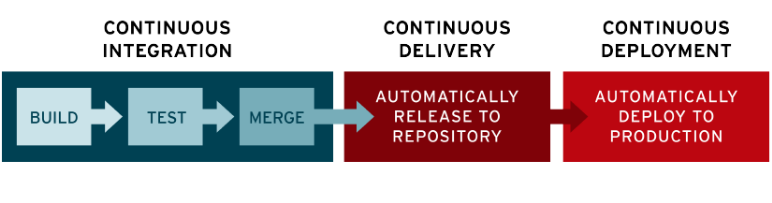
\includegraphics[width=1.0\textwidth]{Red Hat CI CD}
		\caption[\ac{CI}/\ac{CD}]{\ac{CI}/\ac{CD} Prozess als Pipeline\\ \cite{RedHat}}
		\label{fig:RedHat}
	\end{figure}
	
\end{description}

\subsection{Motivation}
\label{subsec:Gründe}
Durch den Review des Codes bestehen zahlreiche Vorteile. Davon sind:

\begin{enumerate}
	\item Das Vermeiden von Fehlern im Quellcode, denn es ist immer sehr umständlich, wenn erst nach einer Weile einen Fehler auftritt, was eine ältere Änderung verursachte.
		Fehler müssen nicht nur, diejenige die das Programm nicht mehr zum Laufen bringen. Die können auch Falsche Schnittstellenspezifikation oder Verletzung von Namenskonventione 
		etc.\ sein.
	\item Fehler die erst beim Kunden auftreten, weil vorher keiner drüber geguckt hat kosten Geld und Reputation.
	\item Die Reviewer können durch lesen der Änderungen lernen.
	\item Der Autor kann durch Review-Kommentare lernen.
	\item Verbesserungsvorschläge und vielmehr.
\end{enumerate}

\subsection{Vorgehensmethoden}
\label{subsec:Vorgehensmethoden}
Es gibt verschiedene Verfahren von Reviews. Die am häufigsten benutzte Verfahren sind:

\begin{itemize}
	\item Ad-hoc: Der Review passiert nur für einen bestimmten Zweck und ist nicht zuvor geplant.
	\item Over–the–shoulder: Der Autor setzt direkt neben dem Reviewer, der die Änderungen kritisiert. Dieses Verfahren ist eine informelle Review.
	\item Email pass-around: Der Autor sendet eine E-Mail mit dem Code zur Überprüfung des Codes an die Reviewer.
	\item Tool-assisted: auch \ac{CRS}. Hier werden Tools benutzt, die die Änderungen je nach Einstellung des Systems an die Rezensenten zum Überprüfen weiterleiten.
	\item Reviewsitzung: Das Team trefft sich regelmäßig, je nach Absprache. Diverse Meinungen werden dargestellt.
	\item Stand Up Meeting: Am Ende des Tages werden die Änderungen diskutiert. Das Team muss nicht unbedingt dabei sein, sondern nur die für die Änderungen zuständig sind.
	\item Planung: Entwickler werden zur Review eingeladen, rollen werden verteilt und die Bedingungen werden festgelegt.
\end{itemize}

\textbf{Nachteile der Methoden die nicht Tool-basiert sind:}
\begin{itemize}
	\item Die Änderungen werden zuerst im Quellcode geschrieben, was Fehler enthalten kann und danach kommt die Review.
	\item Dieser Prozess ist nicht flexibel, denn es fordert die Anwesenheit der für die Änderungen zuständige Personen zusammen mit den Rezensenten.
	\item Es wird für den Review keine Dokumentation erstellt.
\end{itemize}

\subsection{Mögliche Git-Workflows}
\label{sec:Git-Workflows}

Git bietet die Möglichkeit, den Workflow an den Bedürfnisse des Teams anzupassen, daher gibt es unterschiedliche Workflows.
Die Workflows:
\begin{itemize}
	\item Feature-Branch-Workflow
	\item Git-flow-Workflow
\end{itemize}
werden hier vorgestellt.

\subsubsection{Feature-Branch-Workflow}
\label{subsubsec:Feature-Branch-Workflow}

Ziel dieses Workflows, dass ein anderes Branch statt dem Master-Branch (Haupt-Branch) für die Entwicklung von Features und die Review verwendet.
Ablauf: Vom Master-Branch wird einen Zweig erstellt, den der Entwickler zu seiner Arbeitskopie klont. So arbeitet er unabhängig von seinen Kollegen an einem bestimmten Feature und 		sobald er das Feature fertig hat, wird er seine Änderungen mit einem \code{push} in dem abgespaltenen Branch senden. Danach kann der Entwickler je nach Einstellungen des Systems den 	Review starten. Wird der Review z. B. mit einer Pull-Request gemacht werden, soll der Entwickler an dieser Stelle die Pull-Anfrage starten. So können sich die Reviewer die 				Änderungen anschauen, kommentieren und mit dem Autor diskutieren und am Ende diese Änderungen entweder annehmen oder ablehnen. Werden diese Änderungen angenommen, können direkt in 		das Master-Branch zusammengeführt werden \cite{Feature-Branch-Workflow}. Die \cref{fig:Forking-workflow} verdeutlicht diesen Prozess. 

\textbf{Eigenschaften dieses Verfahrens:}
\begin{itemize}
	\item Entwickler arbeiten nicht direkt an dem Haupt-Branch, demzufolge stören sie einander nicht
	\item Jedes Feature ist in einem Feature-Branch gekapselt
\end{itemize}

\subsubsection{Git-flow-Workflow}
\label{subsubsec:Git-flow-Workflow}

"`Der Git-flow-Workflow ist ein Git-Workflow, der von Vincent Driessen auf nvie veröffentlicht und bekannt gemacht wurde. Der Git-flow-Workflow definiert ein strenges Branching-Modell, das um den Release des Projekts konzipiert wurde. Dies bietet einen robusten Rahmen für das Management größerer Projekte.
Git-flow ist hervorragend für Projekte mit einem Release-Zyklus nach Zeitplan geeignet. Mit diesem Workflow werden keine neuen Konzepte oder Befehle hinzugefügt, die nicht auch für 		den Feature-Branch-Workflow erforderlich sind. Stattdessen werden verschiedenen Branches sehr spezifische Rollen zugewiesen, und es wird genau festgelegt, wann und wie die 				Interaktion erfolgen soll. Zusätzlich zu feature-Branches werden einzelne Branches zum Vorbereiten, Warten und Erfassen von Releases verwendet. Dabei kannst du natürlich auch alle 		Vorteile von Feature-Branch-Workflows nutzen: Pull-Anfragen, isolierte Tests und eine effizientere Zusammenarbeit."' \cite{Git-flow-Workflow}

Hier wird also ein anderes Branch (develp-Branch) zusätzlich zum Master-Branch betrachtet. Dieses Branch wird für die Entwicklung verantwortlich sein, indem auf dem Master-Branch 			nur die Versionen zu sehen sind. Die Features werden in abgespaltenen Branchs vom Develop-Branch entwickelt und mit dem develop-Branch nach einer erfolgreichem Pull-Anfrage 				zusammengeführt werden. Sind die Features auf dem develop-Branch soweit für eine neue Version, wird ein Release-Branch vom dvelop-Branch abgespalten, mit dem Release-Branch keine 			Features mehr von anderen Branchs zusammengeführt werden. Dieses Branch sagt einfach "Ich bin die neue Version". Falls das Release-Branch Fehler enthält, kann die Behebung dieser			Fehler wieder in einem anderen Branch geschehen und in das Release-Branch zusammengeführt werden. Funktioniert die Version einwandfrei, wird sie mit dem Master-Branch 						zusammengeführt. Die \cref{fig:Git-flow-Workflow} soll bei der Vorstellung von diesem Workflow helfen.

\begin{figure}[H]
	\centering
	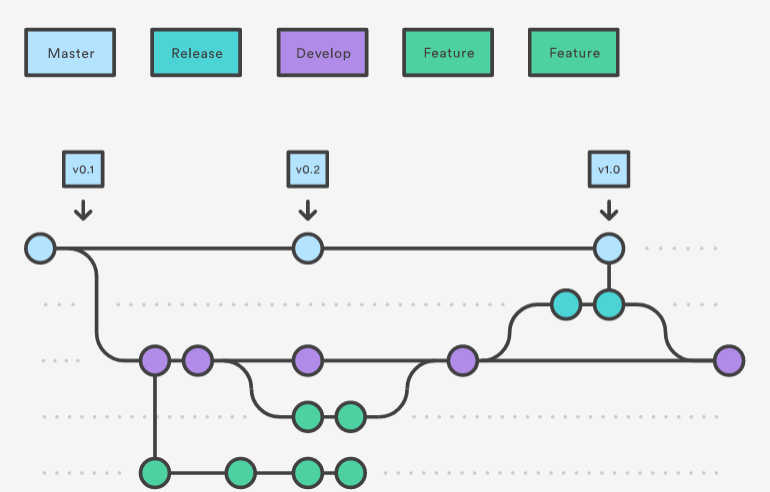
\includegraphics[width=0.9\textwidth]{Git-flow-Workflow}
	\caption[Git-flow-Workflow]{Git-flow-Workflow.\\ \cite{Git-flow-Workflow}}
	\label{fig:Git-flow-Workflow}
\end{figure}
	
\textbf{Eigenschaften dieses Verfahrens:}
\begin{itemize}
	\item Dieser Workflow hat alle Eigenschaften des letzten Workflows im \ref{subsubsec:Feature-Branch-Workflow}
	\item Eignet sich gut für große Projekte, die mehrere Versionen enthalten sollen
	\item Dank des Develop-Branchs und der Release-Branchs hat das Master-Branch eine saubere Historie, da es auf dem Develop-Branchs statt dem Master-Branch entwickelt wird
\end{itemize}


\section{Der Einfluss vom Codereview auf die Softwarequalität in den letzten Jahren}
\label{sec:Einfluss des Reviews}
Smartbear \cite{smartbear} führte im Jahr 2019 mit 1100 Softwareentwickler/Tester, IT- / Betriebsfachleute und Führungskräfte in 35 verschiedenen Branchen eine Umfrage durch. Die Teilnehmer der Umfrage arbeiten in Unternehmen mit unterschiedlichen Größen, von weniger als 25 Mitarbeitern bis zu über 10.000. Ähnliche Umfragen hat Smartbear regelmäßig durchgeführt.

Seit 2016 haben die Befragten identifiziert, dass das Codereview die beste Methode zur Verbesserung der Codequalität ist. Das Unit Testing im Jahr 2019 wurde als zweithöchste Wahl betrachtet und die Daten in der selben Rangliste vom Jahr 2019 zeigen: 25\% der Befragten wählen erneut das Codereview, was in der \cref{fig:Codereview-Softwarequalität} zu sehen ist. Die Wahrnehmung des Codereviews als Schlüssel für eine bessere Softwarequalität wurde durch die Daten vom Jahr 2019 bestätigt.

\begin{figure}[H]
	\centering
	\includegraphics[width=1.0\textwidth]{Codereview-Softwarequalität}
	\caption[Einfluss der Codereview auf die Softwarequalität]{Codereview-Softwarequalität\\ \cite{smartbear}}
	\label{fig:Codereview-Softwarequalität}
\end{figure}

\section{Einfluss der investierte Zeit im Review}
\label{sec:reviewZeit}

Wie im \cref{sec:Einfluss des Reviews} erwähnt, dass Codereview und Softwarequalität eng verbunden sind, so dass es sich lohnt, die Zeit für das Review zu nehmen, um die Qualität des Quelltexts zu verbessern. Die Umfrage von Smartbear zeigt welche sind die wichtigsten Vorteile, die das Review mit sich bringt. Zwar ist das Auffinden von Fehlern die Hauptmotivation, jedoch kann dieser Prozess dabei helfen, die Kommunikation des Teams zu verbessern, das Wissen zu übertragen und die Standardisierung zu erhöhen \cite{smartbear}. 

Die Folgende \cref{fig:Vorteile des Codereviews} stellt die Wichtigste Vorteile des Reviews dar.

\begin{figure}[H]
	\centering
	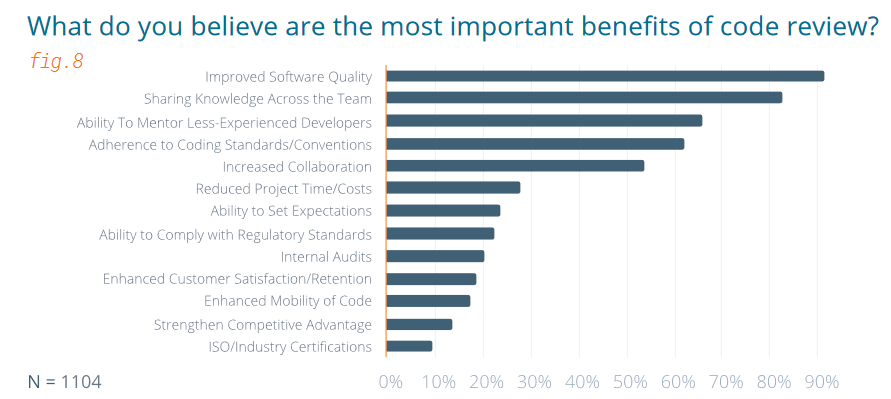
\includegraphics[width=1.0\textwidth]{Vorteile des Codereviews}
	\caption[Vorteile des Codereviews]{Die wichtigsten Vorteile des Codereviews\\ \cite{smartbear}}
	\label{fig:Vorteile des Codereviews}
\end{figure}

Die verbesserte Softwarequalität und die Wissensübertragung im gesamten Team sind seit 2015 die beiden wichtigsten Vorteile \cite{smartbear}.

\subsection{Die vom Programmierer geplante Zeit für das Review}
\label{subsec:reviewerZeit}

Laut der Umfrage von Smartbear (siehe \cref{sec:Einfluss des Reviews}) \textbf{67\%} der Befragten nehmen mindestens wöchentlich am Review teil, während \textbf{42\%} überprüfen den Code täglich.

\subsection{Die am häufigsten für den Review verwendeten Methoden}
\label{subsec:Die am häufigsten verwendete Methoden}

Diese drei Methoden Ad-hoc, Meeting-basiert und Tool-basiert sind die gängigsten Ansätze zum Codereview.
Die entsprechende Daten von der Smartbears Umfrage \cite{smartbear} dieser Methoden verdeutlicht das Balkendiagramm \cref{fig:ReviewZeit} 

\begin{figure}[H]
	\centering
	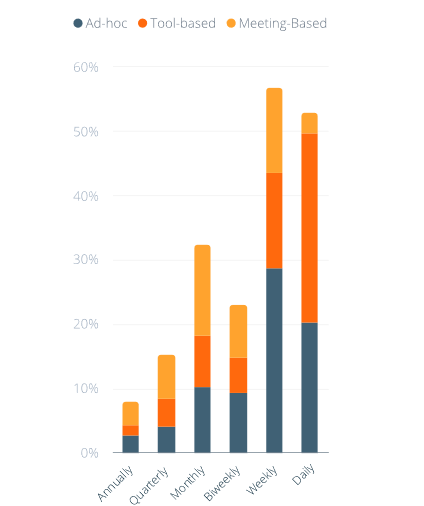
\includegraphics[width=0.7\textwidth]{ReviewZeit}
	\caption[Die Verwendung der bekannten Reviews Methoden]{Die Verwendung der bekannten Reviews Methoden\\\cite{smartbear}}
	\label{fig:ReviewZeit}
\end{figure}

\begin{enumerate}
	\item \textbf{49\%} der Befragten führen mindestens wöchentlich das Review durch Ad-hoc oder Over-the-Shoulder durch, davon sind \textbf{20\%}, die ihr Code auf diese Weise 					täglich überprüfen
	\item \textbf{44\%} der Befragten basiert ihr wöchentliches Review auf Tools, davon sind \textbf{29\%}, die das Review mit Tools täglich machen
	\item \textbf{16\%} der Befragten organisieren ein Meeting wöchentlich für das Review, davon sind \textbf{3\%}, die das Review auf diese Weise täglich durchführen
\end{enumerate}

\pagebreak

\section{Codereview-Tools}
\label{sec:Coderview-Tools}

Es gibt 4 Bereiche, mit denen Entwicklern ihren Code überprüfen.

\begin{itemize}
	\item \textbf{Repository-Verwaltungstools:} Diese Tools sind für die Verwaltung von Repositories zuständig. Entwickler können das Review durchführen, indem sie das Pull Request an
		Teammitglieder senden oder auch durch andere Verfahren wie der Fall bei Helix Teamhub im \cref{subsec:HelixTeamHub}
		Beispiele dafür sind z.B.:
		\begin{itemize}
			\item Bitbucket \cref{subsec:Bitbucket}
			\item Github \cref{subsec:Github}
		\end{itemize}
	
		Smartbears Umfrage zufolge verwenden \textbf{69\%} der Befragten Repository Tools als Teil ihres Codereviews, unabhängig davon, ob sie das Review durch eine Pull Request 					durchführen oder in ein spezielles Peer Codereview Tool oder statisches Analysetool integrieren. Das bildet ein deutlicher Anstieg von \textbf{42\%} im Jahr 2018 							\cite{smartbear}

	\item \textbf{\ac{IDE}:} Wie z.B. Visual Studio\footnote{https://visualstudio.microsoft.com} bietet die Möglichkeit, direkt in der Umgebung das Review zu starten

	\item \textbf{Statische Analysetools:} Ein Beispiel dafür ist SonarQube\footnote{https://www.sonarqube.org}. Es ist eine Plattform, die automatisierte Regeln für die statische Code-			Analyse definieren und benachrichtigt den Entwickler von seiner Pull Request, die durch Repository-Verwaltungstools erstellt wurden

	\item \textbf{Peer-Codereview-Tools:} Beispiele sind: Crucible im \cref{subsec:Crucible} und Gerrit im \cref{subsec:Gerrit}. Das Hauptziel solcher Tools ist, einen einfachen und 				unkomplizierten Review anzubieten. Sie können kein Repository verwalten, haben aber andere Eingenschaften beispielsweise Änderungsvergleich anzeigen
\end{itemize}

\subsection{Codereview-System}
\label{subsec:CRS}

Ein Codereview-System ist ein allgemeiner Begriff, der ein Tool beschreibt, das fähig ist, die Entwickler die Möglichkeit anbietet Codereview durchführen zu können und diesen Review zu steuern. Dieses System kann ein Repository Verwaltungstool, Statisches Analysetool, IDE oder ein Peer-Codereview-Tool sein. Beispiele dafür sind im \cref{sec:CRS-Git}.

\subsection{Kriterien \& Erwartungen an das System}
\label{sec:kriterien}

Folgende Eingenschaften sind die Kriterien, die in Betracht bei der Vorstellung von allen \acp{CRS} genommen werden sollen:

\begin{itemize}
	\item Es soll das \ac{VCS} Git unbedingt unterstützen
	\item Die Unterstützung vom \ac{VCS} \ac{SVN} ist ein Bonus
	\item Es soll den Änderungsvergleich sowohl inline als auch Side-by-side deutlich darstellen können
	\item \ac{CI}/\ac{CD} Tools sollen in den Workflow eingebaut werden können oder in dem System integrieren sein
	\item Das System kann auf dem eigenen Server gehostet werden
	\item Das System kann die Review-Kommentare nach Beenden des Reviews automatisch mit dem Haupt-Repository Zusammenführen
	\item Review-Kommentare sind auf Zeilenebene möglich
	\item Zugriffsverwaltung ist ein Vorteil
\end{itemize}

\section{Codereview-Tools}
\label{sec:Coderview}

\unsure{IDE Tools und  Static analysis tools erwähnen}
\unsure{Beschreibe die Arten von CRSs 1) post-commit 2) pre-commit 3) pull-requests}
\blindtext
\blindtext

\section{Codereview-Systeme, die Git unterstützen}
\label{sec:CRS-Git}

\subsection{Bitbucket}
\label{subsec:Bitbucket}

Bitbucket ist ein Quellcode-Management-System der das \ac{VCS} Git unterstützt. Bitbucket unterstützte nach seinem Entwurf als \ac{VCS} nur Mercurial. Erst 3 Jahren später wurde um die Unterstützung von Git erweitert. Am 1. Juni 2020 wurde die Unterstützung von Mercurial vollständig eingestellt.

\begin{itemize}
	\item \textbf{Art der Review}: \textit{pre- and post-commit} Und die erfolgt durch eine Pull-Anfrage.
	\item \textbf{Entwickler}: Bitbucket wurde 2007 vom Jesper Nøhr entwickelt und 2010 von Atlassian \footnote{\url{https://bitbucket.org/}}
		 gekauft. 
	\item \textbf{Reviews Workflow}: Eine Pull-Request kann in 3 verschiedenen Weisen gemacht werden:
		\begin{itemize}
			\item Feature-Branch-Workflow.
			\item Git-flow-Workflow.
			\item Forking-Workflow.
		\end{itemize}
\end{itemize}

Die Abbildung \ref{fig:Forking-workflow} zeigt die Forking-Workflow mit Pull-Anfrage.

\begin{figure}[H]
	\centering
	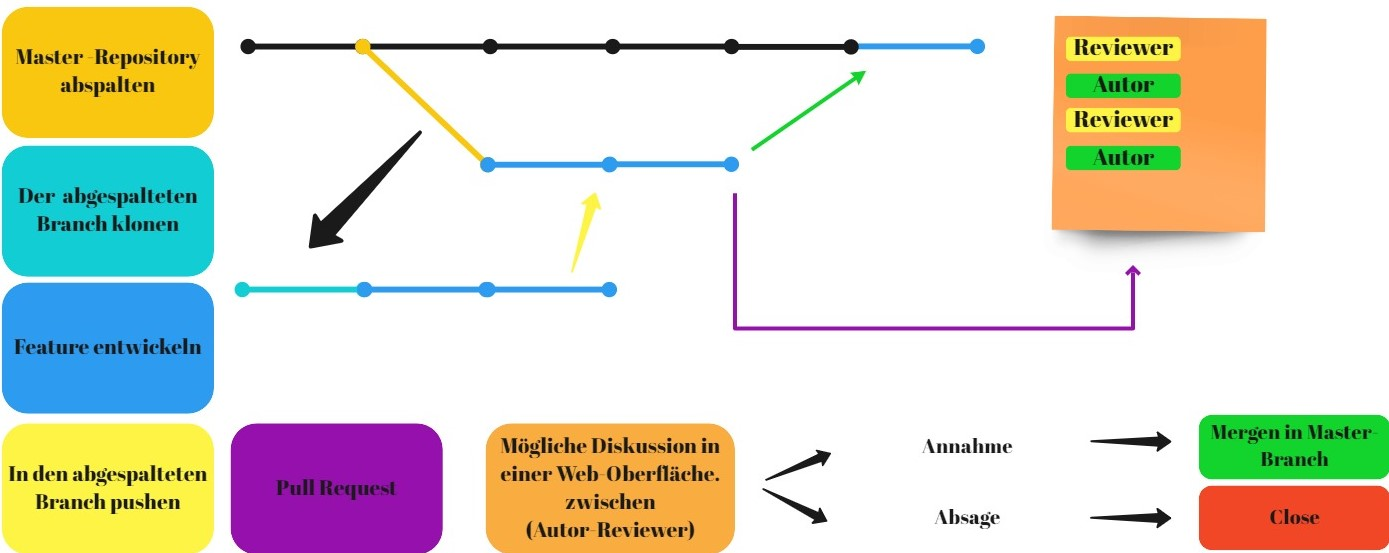
\includegraphics[width=1.0\textwidth]{Bitbucket_Forking-Workflorw}
	\caption[Bitbuckets Ablauf]{Pull-Request.\\ Quelle: eigene Darstellung}
	\label{fig:Forking-workflow}
\end{figure}		  

\begin{description}
	\item [Vorteile:] \hfill
	\begin{enumerate}
		\item Unbegrenzte Anzahl von private Repositories.
		\item Hosting in Cloud oder auf eigenem Server.
		\item \ac{CI}/\ac{CD} sind in Bitbucket integriert.
		\item Erstellen von einer Merge-Checkliste mit zugeordneten Genehmigern.
		\item Für kleine Teams bis 5 Personen bestehen keine Kosten für das Hosten auf Bitbuckets Server.
	\end{enumerate}
	
	\item [Nachteile:] \hfill
	\begin{enumerate}
		\item Es besteht keine Möglichkeit, um bestehende gemergte commits zu reviewen.
		\item Review ist nur vor dem Zusammenführen von einem Feature-Branch mit dem Master-Branch Möglich.
		\item Um zu hosten auf Bitbucketsever steht für mehr als 5 Personen einen monatlichen Beitrag und für Self-hosten (auf eigenem Server) besteht eine einmalige Zahlung. Der 
			Preis für beide Varianten variiert je nach Personenanzahl.
	\end{enumerate}
\end{description}

\subsection{Crucible}
\label{subsec:Crucible}

Crucible ist eine webbasierte Anwendung, die eine unkomplizierte, formelle Codereview anbietet. Sie unterstützt die \acp{VCS} SVN, Git, Mercurial, CVN, perforce.

\begin{itemize}
	\item \textbf{Art der Review}: \textit{pre- and post-commit}
	\item \textbf{Entwickler}: Crucible ist ein Atlassian Produkt.
	\item \textbf{Workflow}: Es gibt verschiedene Weisen, wie man eine Review in Crucible durchführen kann. Allerdings werden sich diese nach den an der Review beteiligten Personen
		 unterscheiden, diese sind:
		\begin{itemize}
			\item Der Moderator. Er ist die Person, die die Review startet und für das Schließen der Review verantwortlich ist.
			\item Die Reviewer
			\item Der Autor
		\end{itemize}
		Beispiele:
		
		\begin{enumerate}
			\item One-to-One Reviews: Der Autor startet die Review (Der Autor ist also in diesem Workflow der Moderator), danach kommentiert der Reviewer und der Autor kann auf diese
				Kommentar reagieren. Das kann sich mehrmals wiederholen bis die Review fertig ist und der Autor diese schließt.\\
				Die Abbildung \ref{fig:one-to-one-workflow} beschreibt diesen Workflow.
				\begin{figure}[H]
					\centering
					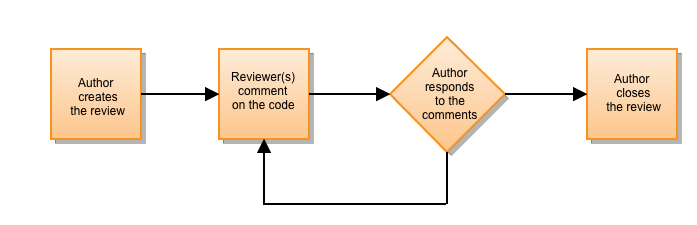
\includegraphics[width=1.0\textwidth]{one-to-one-review}
					\caption[Crucible: one-to-one-review]{Crucible Ablaufsmöglichkeit,\\ Quelle: \cite{Crucible}}
					\label{fig:one-to-one-workflow}
				\end{figure}
				
			\item Formal group reviews: Der Autor startet die Review und lädt die Reviewer ein. So können die Reviewer diese diskutieren und dementsprechend bekommen die Reviewer 
				die Antworten vom Autor (Der Autor ist in dem Fall auch der Moderator). Jeder Diskussionspunkt wird vom Moderator festgelegt. So bald die Review zu Ende kommt,
				fasst der Moderator die Review zusammen und schließt sie.\\
				Die Abbildung \ref{fig:Formal-group-review} zeigt diesen Ablauf.
				\begin{figure}[H]
					\centering
					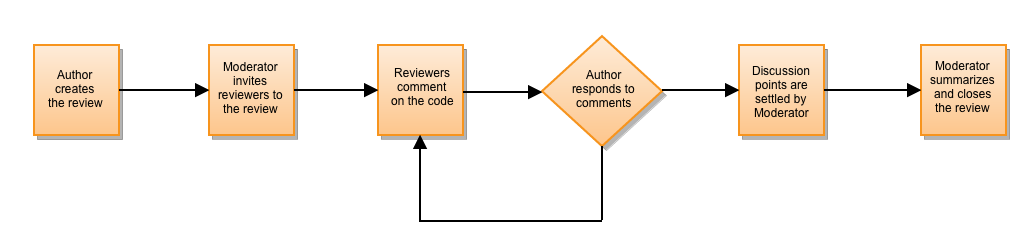
\includegraphics[width=1.0\textwidth]{Formal-group-reviews}
					\caption[Crucible: Formal group review]{Crucible Ablaufsmöglichkeit,\\ Quelle:\cite{Crucible}}
					\label{fig:Formal-group-review}
				\end{figure}
		\end{enumerate}
		
\end{itemize}

\begin{description}
	\item [Crucibles Vorteile:] \hfill
	\begin{enumerate}
		\item Review des Inhalts ist flexibel.
		\item Diskussionsrunden um in Bestimmten Quelltextzeilen oder ein bestimmtes Commit sowie einen gesamten Änderungssatz zu Kommentieren.
		\item Nachverfolgen, Maßnahmen ergreifen in Bezug auf das, was der Autor wichtig findet.
		\item Ansicht vom Reviewstatus und wer möglicherweise Überprüfungen aufhält.
		\item Berichte über Stellen im Quelltext, die noch nicht überprüft wurden.
		\item unterstützt nicht nur Git sonder SVN auch.
	\end{enumerate}
	
	\item [Crucibles Nachteile:] \hfill
	\begin{enumerate}
		\item Die Review muss manuell in Git eingefügt werden(Mergen ist nicht möglich).
		\item Schwer zu erzwingen.
	\end{enumerate}
\end{description}

\subsection{Helix TeamHub}
\label{subsec:HelixTeamHub}

Helix TeamHub ist eine webbasierte Plattform, die Hosten und Management von Repositories ermöglicht. Sie unterstützt Mercurial, Git, SVN, Ivy und mehr.

\begin{itemize}
	\item \textbf{Art der Review}: \textit{pre- and post-commit}.
	\item \textbf{Entwickler}: Perforce. 
	\item \textbf{Reviews Workflow}: Die Review kann in Helix Teamhub eingerichtet werden, so kann das Mitglied, das die Review erstellte, entscheidet, wer die Reviewer
		 sind und welche Änderungen in welchem Branch überprüft werden sollen.
		 Ein Beispiel für einen möglichen Workflow:
		 
		  Git-Feature-Branch-Workfow: Der Ablauf ähnelt sich dem Feature-Branch Workflow von Bitbucket in Abschnitt \ref{subsec:Bitbucket}.
		  Es wird zuerst ein Projekt erstellt und zu diesem Projekt wird ein Repository hinzugefügt. Durch Git wird ein Branch in diesem Repository
		  erstellt. Der Entwickler arbeitet an diesem Branch. Sobald er eine Review braucht, erstellt er eine. In den Einstellungen sucht man den Branch aus, dann werden Reviewer
		  ausgewählt. In der Review sind die Kommentare auf Zeilenebene möglich. So bekommt der Autor Antworten und Verbesserungsvorschläge. Sobald die Review fertig ist,
		  können die Änderungen automatisch in den Master Branch zusammengeführt werden, was sich durch einen Klick erfolgen lässt. 
\end{itemize}

\begin{description}
	\item [Vorteile:] \hfill
	\begin{enumerate}
		\item Workflows sind flexibel, so dass die Administratoren diese einrichten können.
		\item Schnelle Übersicht über alle Branchs eines Repositorys.
		\item Zugriffsverwaltung, so kann sich der Admenstrator entscheiden, wer an einem repository arbeitet und welche Rechte hat.
		\item Side-by-side Änderungsvergleich.
		\item Der Prozess der Review kann kontrolliert werden. Die Review kann auf bestimmte Personen beschränkt werden.
		\item Mergen von Reviews erfolgt automatisch.
		\item Helix Teamhub unterstützt \ac{CI}/\ac{CD} Tools.
		\item Kostenlos für Teams bis 5 Mitglieder.
	\end{enumerate}
	
	\item [Nachteile:] \hfill
	\begin{enumerate}
	\item Für die kostenlose Variante steht totale Speichergröße von 1GB in Cloud zu Verfügung.
	\item Hosten auf eigenem Server ist nicht möglich.
	\item Die Abspeicherung von Daten auf dem Server variiert je nach dem jährlichen Beitrag.
	\end{enumerate}
\end{description}


\subsection{Gerrit}
\label{subsec:Gerrit}

Gerrit ist ein \ac{CRS}, das sich von den anderen \acp{CRS} stark unterscheidet. Gerrit ist ein \ac{CRS}, das nur mit dem \ac{VCS} Git arbeitet und Benutzers Änderungen nicht direkt ohne Kontrolle in den Server gepusht werden lässt. Außerdem ist Gerrit auch eine Webbasierte Anwendung, in der die Review geschieht.

\begin{itemize}
	\item \textbf{Art der Review}: \textit{pre-commit}
	\item \textbf{Entwickler}: Google.
	\item \textbf{Workflow}: Gerrit hat nur einen Ablauf für den Review, der nach diesen Schritten erfolgt:
		\begin{enumerate}
			\item Projekt für das Repository erstellen. Für die Erstellung vom Gerrit-Projekt gibt es 4 Methoden:
			\begin{itemize}
				\item Direkt im Gerrits Web-Plattform.
				\item via REST endpoint
				\item via SSH command
				\item Manuell durch git
			\end{itemize}
			Hinweis: Nicht jeder Benutzer kann ein Gerrits Projekt erstellen, denn das braucht Administratorrechte.		
			
			\item Features entwickeln, dann die commiten und pushen. In diesem Fall pusht man die Änderungen nicht in den Master Branch, sondern in einen Gerrits Branchen.
				Gerrit benutzt Dieser Branch für die Review. Dementsprechend kommt man mit \textit{git diff} (git Befehl, um alte und neue Änderungen zu vergleichen) zum Vergleich
				zwischen den Änderungen im Arbeitsverzeichnis und den Änderungen auf der Gerrits Branche.
			\item Nach pushen wird einen Link erzeugt, den zur Webseite führt. Auf dieser Webseite kann der Autor: 
			\begin{itemize}
				\item Diffs anzeigen lassen.
				\item Reviewer hinzufügen.
				\item Kommentare, Anmerkungen an bestimmten Code-Zeilen für die Reviewer hinterlassen.
			\end{itemize}
			Die Abbildung \ref{fig:Gerrit-Reviews Webseite} soll einen allgemeinen Überblick über die Webseite geben.
			
			\begin{figure}[H]
				\centering
				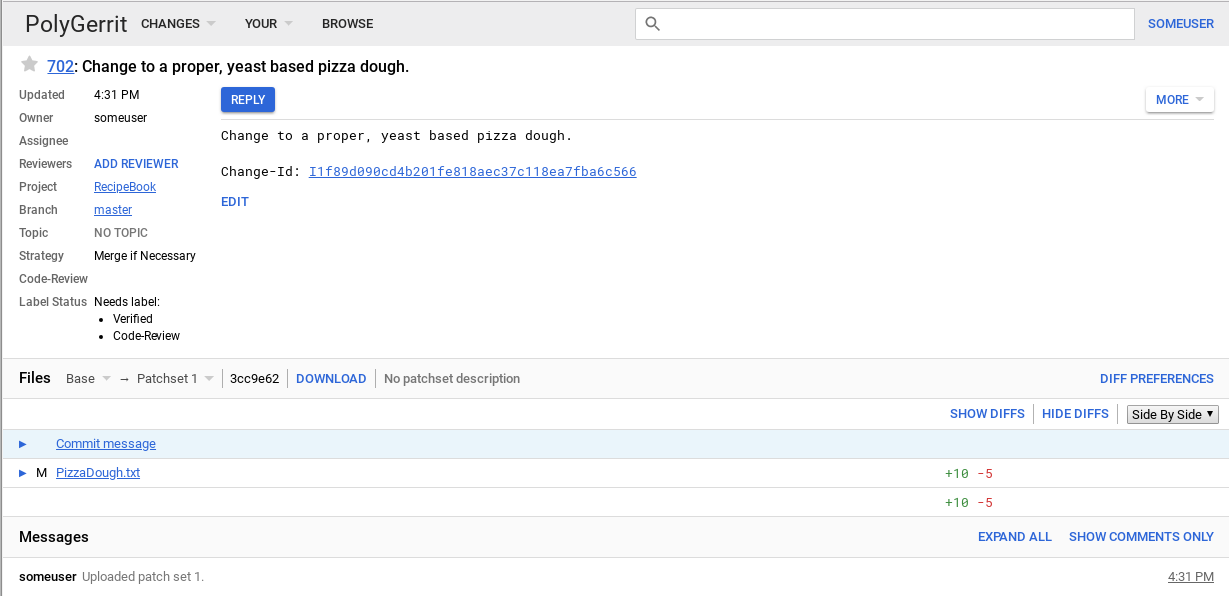
\includegraphics[width=0.9\textwidth]{Gerrit-Reviews Webseite}
				\caption[Gerrit]{Reviews Webseite,\\ Quelle: \cite{Gerrit}}
				\label{fig:Gerrit-Reviews Webseite}
			\end{figure}
						
			\item Die Reviewer können entweder die Review manuell finden oder bekommen die eine E-Mail (wenn sie vom Autor als Reviewer gemerkt sind), dass eine Review
				 gestartet wurde. Die Reviewer schauen die Änderungen, antworten auf sie und am Ende bewerten sie. Die Bewertung ist in Gerrit vorgeschrieben.
				 Dann passiert Folgendes:
				 \begin{itemize}
				 	\item Sind die Änderungen fehlerhaft oder fehlt etwas, was der Autor beachten musste, so fordern die Reviewer den Autor, die Änderungen zu bearbeitet
				 		und nochmal in den Gerrits Branch zu pushen.
				 	\item Erfüllen die Änderungen die Anforderungen, So ist die Review geschlossen.
				 \end{itemize}
			\item Darüber hinaus fragt Gerrit nach Bestätigung, dass die Änderungen getestet wurden, dass die also funktionieren. Testen kann entweder 
			\begin{itemize}
				\item Manuell. Die Änderungen fetchen und lokal testen
				\item Oder durch Nutzen von \ac{CI} Tools.
			\end{itemize}
			\item So bald die Review fertig ist und die Features getestet wurden, werden die Änderungen einschließlich der Review je nach den Projekts Einstellungen in
				den Master Branch gepusht.
		\end{enumerate}
		
\end{itemize}

\begin{description}
	\item [Gerrits Vorteile:] \hfill
	\begin{enumerate}
		\item Gerrit kann multiple Repositories beaufsichtigen.
		\item Clean history \unsure{Erkläre warum (git push --f)}
		\item Jedes Repository kann unendliche Anzahl von Branchs enthalten.
		\item Automatisches Mergen mit dem Git-Repository nach Überprüfung der Änderungen ist möglich.
		\item \ac{CI}/\ac{CD} können in den Workflow eingebaut werden.
		\item Benutzerfreundliche Webschnittstelle zum Reviewen.
		\item Kostenlos \& Open-Source-Projekt.
	\end{enumerate}
	
	\item [Gerrits Nachteile:] \hfill
	\begin{enumerate}
		\item Mit Gerrit ist die Review und das Testen der neuen Änderungen Pflicht.
		\item Nur Administratoren können Projekte in Gerrit hinzufügen.
		\item Gerrit arbeitet ausschließlich mit Git.
	\end{enumerate}
\end{description}

\subsection{RhodCode}
\label{subsec:RhodeCode}

RhodCode ist ein Quellcode-Management, das die \acp{VCS} Git, Mercurial unterstützt. Es ist eine webbasierte Plattform also bietet auch eine Web-Schnittstelle, in der die Review geschieht.
RhodCode bietet eine freie Edition „RhodeCode CE“ (Community Edition) sowie zwei kostenpflichtige Editions „RhodeCode EE“ (Enterprise Edition) und RhodeCode Cloud (Beta).

\begin{itemize}
	\item \textbf{Art der Review}: \textit{pre- and post-commit}
	\item \textbf{Entwickler}: RhodeCode.
	\item \textbf{Workflow}:
	\begin{itemize}
		\item Die Review kann durch eine Pull-Anfrage gestartet werden. Die Abbildung \ref{fig:Forking-workflow} vom Abschnitt \ref{subsec:Bitbucket} zeigt den Ablauf
			eine Pull-Anfrage. Also der Entwickler arbeitet in einem vom Master-Branch abgespalteten-Branch macht Änderungen und sendet eine Pull-Anfrage so bald er fertig ist. 
			So Geschieht die Review dementsprechend vor dem Mergen mit dem Master-Branch.
		\item Oder kann der Reviewer sich die Änderungen in Commits-Historie anschauen und bestimmte Code-Zeile kommentieren und den Autor erwähnen, indem er seinen Namen nach einem 
			\textbf{@} schreibt. So bekommt der Autor eine E-Mail, dass jemand seine Änderungen überprüft hat.
	\end{itemize}
\end{itemize}

\subsubsection{RhodeCode CE}
\label{subsubsec:RhodeCode CE}

\begin{description}
	\item [Vorteile] \hfill
		\begin{enumerate}
			\item Ein kostenloses- und Opensource-Projekt.
			\item Unbegrenzte Anzahl von Benutzern.
			\item Benutzerzugriffskontrolle.
			\item Dateisuche in allen Repositories sowie Volltextsuche \& Indizierung vom Quellcode.
			\item Grundlegende Integrationen einschließlich E-Mail, Slack und Hipchat.
		\end{enumerate}
	\item [Nachteile] \hfill
		\begin{enumerate}
			\item Die diffs lassen sich nur inline angezeigt werden.
			\item Einschränkungen der Review sind nicht möglich.
			\item RhodeCode CE unterstützt keine \ac{CI}/\ac{CD} Tools.
			\item Hosting geht nur auf eigenem Server.
		\end{enumerate}
\end{description}

\subsubsection{RhodeCode EE}
\label{subsubsec:RhodeCode EE}

\begin{description}
	\item [Vorteile] \hfill
		\begin{enumerate}
			\item Hat alle Feature der RhodeCode CE im Abschnitt \ref{subsubsec:RhodeCode CE}.
			\item Die diffs lassen sich inline oder side-by-side angezeigt werden. 
			\item Die Review unterstützt Live-Chat für das Quellcode vor Ort sowie Feedback in allen Repositories.
			\item Regeln für Review stellen. z. B. Wer die Änderungen überprüfen kann.
			\item Sperren von Repositories; Admins können Repositories sperren, so dass keine Änderungen mehr von anderen Benutzern in die Master-Branche gepusht sind.
			\item Dateien, Projekte und Repositories ordnen, strukturieren und unbegrenzt \, verschachteln.
			\item Unterstützt die Migration vom \ac{VCS} SVN zu Git.
			\item RhodeCode EE unterstützt \ac{CI}/\ac{CD} Tools.
			\item Volltextsuche nach Umgebungen mit sehr großen Codebasen. Es kann Terabyte von Daten verarbeiten.
		\end{enumerate}
	\item [Nachteile] \hfill
		\begin{enumerate}
			\item Verfügbar nur für mindestens 10 Benutzer mit einem jährlichen Beitrag von 75\$ pro Benutzer.
			\item Kein open-source Projekt.
			\item Hosting geht nur auf eigenem Server.
		\end{enumerate}
\end{description}

\unsure{RhodeCode Cloud (Beta) ?}

\subsection{Github}
\label{Github}

Github ist eine webbasiert Plattform für das Management vom Quelltext. Github arbeitet ausschließlich mit dem \ac{VCS} Git. Es bietet die Gelegenheit, unbegrenzte Anzahl von public/private Repositories (Private Repositories erst seit 8. Januar 2019) auf Githubs Server zu hosten. Außerdem gehört Github seit Juni. 2018 Microsoft.

\begin{itemize}
	\item \textbf{Art der Review}: \textit{pre- and post-commit}
	\item \textbf{Entwickler}: Tom Preston-Werner, Chris Wanstrath, P. J. Hyett.
	\item \textbf{Workflow}: Die Review funktioniert in Github durch eine Pull-Anfrage, wie beim Bitbuckets Workflow in \ref{subsec:Bitbucket} arbeitet der Entwickler an einem
		speziellen Branch, macht Änderungen und startet eine Pull-Anfrage und wählt die Reviewer, die eine Nachricht bekommen, dass sie zur Überprüfung gefragt sind. Nach Annahme der
		Änderungen, können diese automatisch mit dem Master-Branch zusammengeführt werden.
\end{itemize}

Github bietet 3 Pläne. Davon werden nur 2 vorgestellt:

\subsubsection{Github Free}
\label{subsubsec:Free}

Die Kostenlose Variante für die Community.
\begin{description}
	\item [Vorteile:] \hfill
	\begin{enumerate}
		\item Seit 14.~April 2020 kann unbegrenzte Anzahl von Benutzern nicht nur an öffentlichen Repositories zusammenarbeiten sondern auch an privaten Repositories.
		\item Kostenlose Nutzung von Quellcode-Test-Tools(\ac{CI}/\ac{CD}) für die öffentlichen Repositories und 2000 Minuten im Monat für private Repositories
		\item 500 MB Speicher für GitHub-Pakete und unbegrenzte Speicher für öffentliche Repositories
		\item Codereview-Tools: Änderungsvergleich anzeigen lassen, Pull-Anfragen
		\item Automatisches Zusammenführen nach Genehmigung der Review
	\end{enumerate}
	\item [Nachteile:] \hfill
	\begin{enumerate}
		\item Einschränkungen auf Branchen sind nicht möglich
		\item Die Review kann nicht auf bestimmte Benutzer beschränkt werden
		\item Öffentliche Repositories haben mehr Features als die private Repositories
	\end{enumerate}
\end{description}

\subsubsection{Github Team}
\label{subsubsec:Team}

\begin{description}
	\item [Vorteile:] \hfill
	\begin{enumerate}
		\item Enthält alles was die Kostenlose Variante \ref{subsubsec:Free} kann
		\item 3,000 Minuten im Monat für die Nutzung von Quellcode-Test-Tools für private Repositories
		\item 2 GB Speicher für GitHub-Pakete
		\item Informelle Pull-Anfragen starten, bevor man die formelle Überprüfung durchführt
		\item Einschränkungen für das Zusammenführen von Branchen erzwingen
		\item Anforderung zur Review durch ausgewählte Benutzer
		\item Rechte für die Branchen geben, so können nur bestimmte Benutzer an einer bestimmten Branche arbeiten
	\end{enumerate}
	\item [Nachteile:] \hfill
	\begin{enumerate}
		\item Monatlichen Beitrag in Höhe von 4\$ pro Benutzer
		\item Hosten auf eigenem Server ist in diesem Paket nicht erhältlich
	\end{enumerate}
\end{description}

Außerdem hat Github eine Desktop-Anwendung, mit der verschiedene Operationen wie (Diffs anzeigen, fetchen, mergen, pushen) ohne Command-line durchgeführt werden können.


\section{Testphase}
\label{sec:testphase}

Zum Testen vom Reviews Workflow und von anderen Funktionen der ausgesuchten Systeme \cref{sec:Ausgesuchte Systeme}, wird diese Arbeit, die bereits mit Git versioniert und auf dem Server der Abteilung gehostet wurde, verwendet, deswegen wird sie in den nächsten Bildern erscheinen. Die zwei Systeme werden ebenfalls auf Server installiert. Der Reviewer wird der Experte Björn Schäpers \cite{Bjoern} sein.

\subsection{Bitbucket}
\label{subsec:Test_Bitbucket}

In den folgenden Unterabschnitten werden die Varianten:
\begin{itemize}
	\item Bitbuckets Webanwendung. Hosten auf Bitbuckets Server.
	\item Self-hosten mit Bitbucket-Server.
\end{itemize}

vorgestellt und miteinander verglichen.

\subsubsection{Hosten auf dem Server des Anbieters}
\label{subsubsec:Bitbucket-Cloud}

Für den Beginn Verlangt die Webanwendung vom Bitbucket nur eine Anmeldung und schon kann man anfangen, Projekte zu erstellen, in denen die Repositories geklont oder neue erstellt werden können. In dieser Anwendung können auch Funktionen durchgeführt werden, die man mit dem Befehl Line von Git macht. Wie beispielsweise ein neues Branch erstellen, wie in \cref{fig:Bitbucket-Branch-erstellen} zu sehen ist oder ein Repository klonen.

\begin{figure}[H]
	\centering
	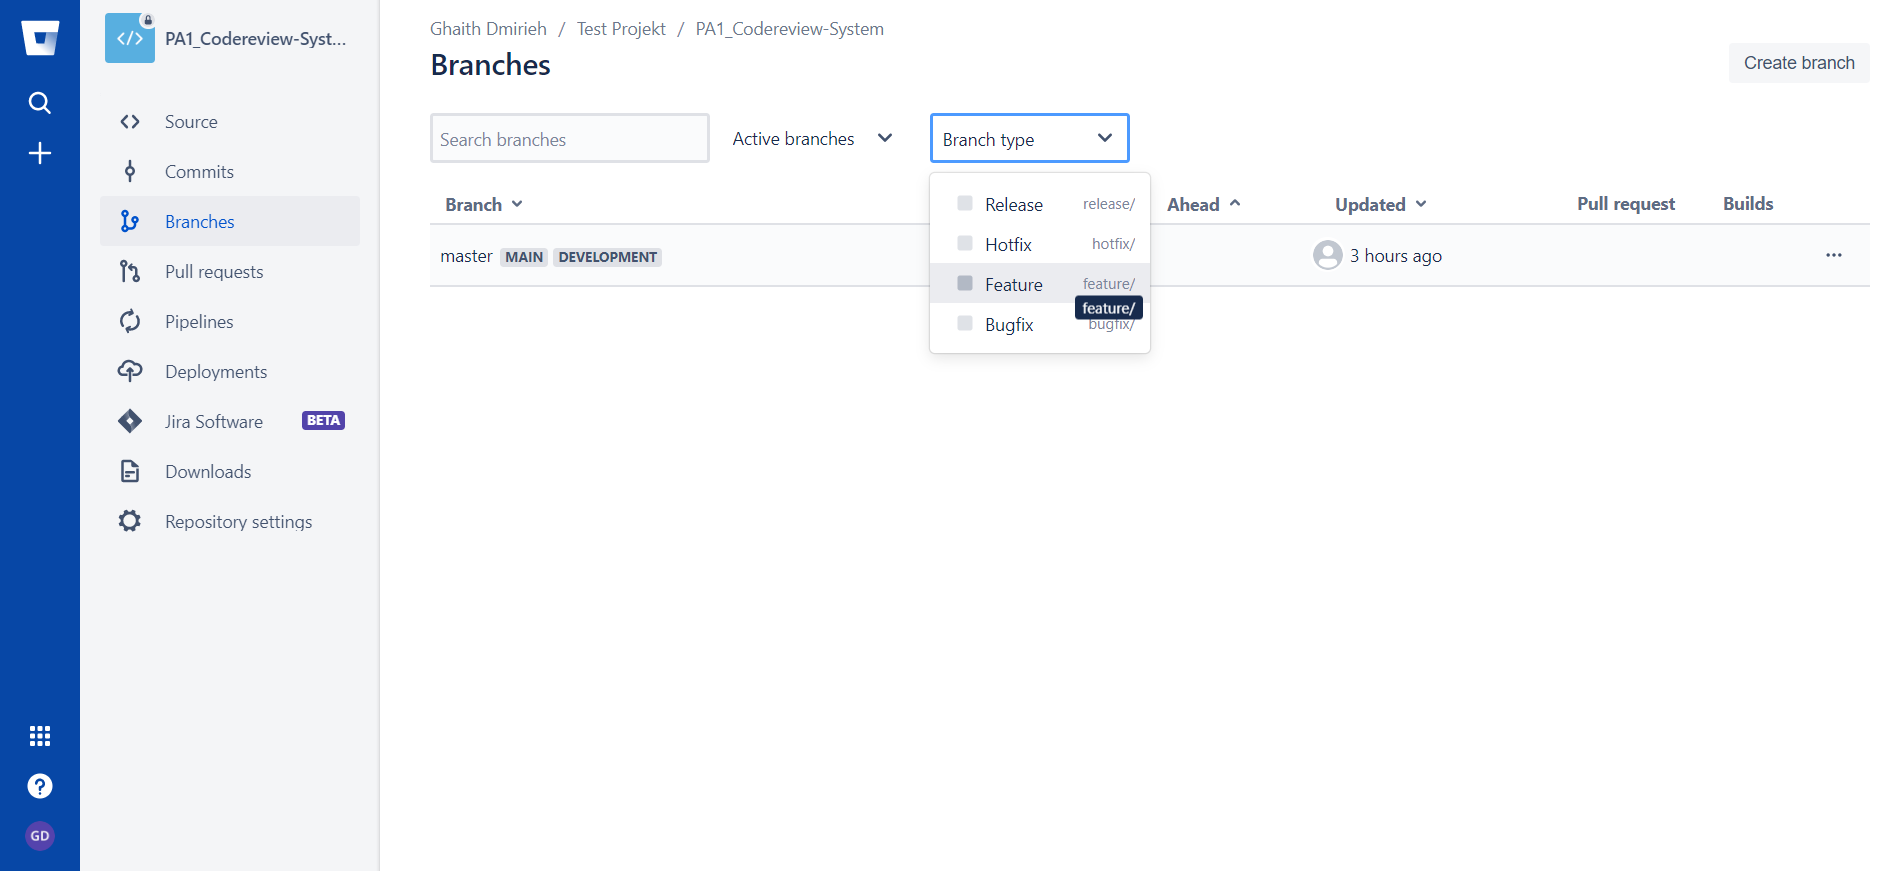
\includegraphics[width=1.0\textwidth]{Bitbucket-Branch-erstellen}
	\caption[Branch auf Bitbuckets Anwendung erstellen]{Ein neues Branch erstellen\\Eigener Screenshot}
	\label{fig:Bitbucket-Branch-erstellen}
\end{figure}

Die Webanwendung ist im Stande, die Änderungsvergleich von jedem commit sowohl inline als auch side-by-side anzuzeigen. Ein Beispiel dafür ist die \cref{fig:Diffs_side-by-side}.

\begin{figure}[H]
	\centering
	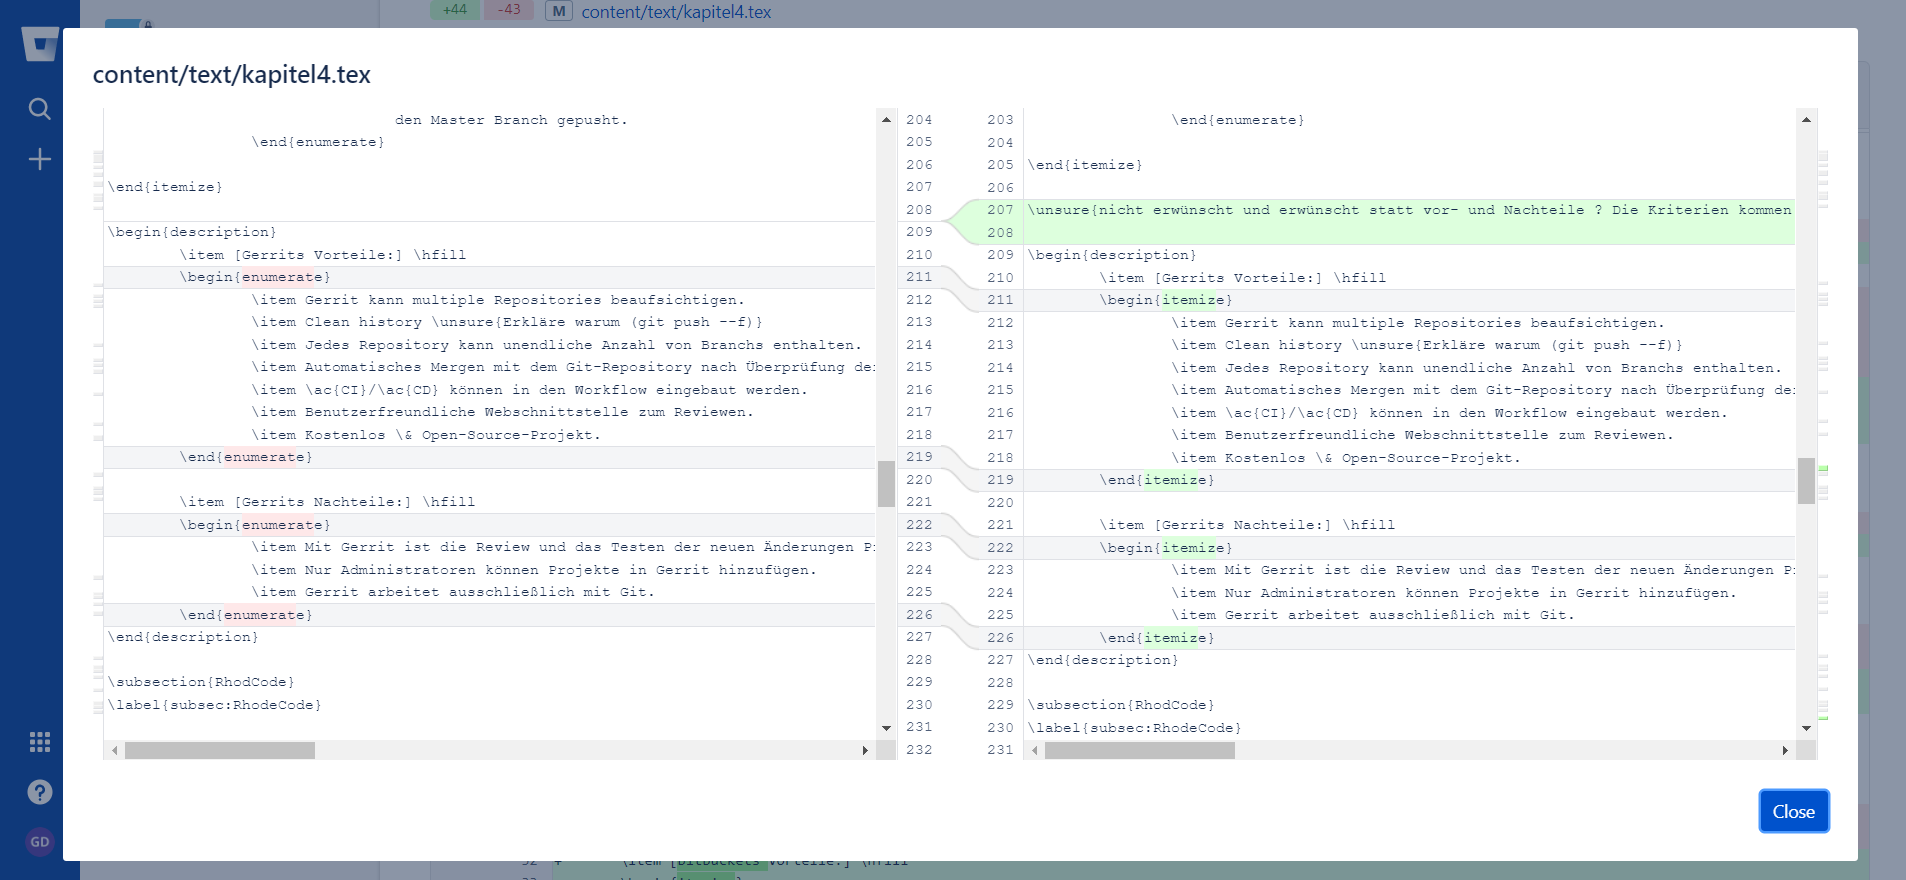
\includegraphics[width=1.0\textwidth]{Bitbucket side-by-side diffs}
	\caption[Bitbuckets Webanwendung side-by-side Änerungsvergleich]{Diffs side-by-side\\Eigener Screenshot}
	\label{fig:Diffs_side-by-side}
\end{figure}

Im Gegensatz zu anderen Tools wird hier nur die Stelle, die geändert ist, markiert und nicht die ganze Zeile, die dazu gehört, was bei einer klaren Übersicht beiträgt.
Das Erstellen von Pull Request für den Feature Branch Übernimmt die Benutzer die an diesem Branch arbeiten. Beim Erstellen das Pull Requests wird der Feature Branch und der Ziel Branch ausgesucht und die Reviewer werden vom Autor ausgewählt. Die Beschreibung vom Pull Request wird die Nachrichten der Commits, die in dem Feature Branch eingecheckt wurden. Diese Beschreibung kann aber geändert werden.

Die Reviwer können das Pull Request auf Zeilen Ebene kommentieren, Todos erstellen \footnote{Allerdings nur nach dem Kommentar}. Direkte Änderungen am Quelltext, die der Autor annehmen kann, sind nicht möglich \footnote{Zumindest mit der freien Version von Bitbucket-Cloud}. Benutzer dieser Cloud-Version können keine Einschränkungen auf das Pull Request stellen, so kann der Feature Branch mit dem Ziel-Branch vom Autor zusammengeführt wird ohne ,dass die Reviewer das Pull Request zustimmen oder die von den Reviewern erstellte Todos gemacht zu haben.

\subsubsection{Self-Hosten}
\label{subsubsec:Bitbucket-self-host} 

Die Installation von Bitbucket-Server mit der Versionsnummer 7.2.3 erfolgte durch eine ZIP-Datei. Ein Verzeichnis für die Projekte und deren Repositories muss manuell erstellt werden und auf es in der Konfiguration-Datei \textit{set-bitbucket-home.sh} verwiesen werden, diese ist im Verzeichnis \textit{/atlassian-bitbucket-7.2.3/bin} zu finden. Wenn es kein Script für das Starten bzw. Stoppen von Bitbucket-Server erstellt wird, sind die ausführbare Dateien \textit{start-bitbucket.sh} und \textit{stop-bitbucket.sh} dafür verantwortlich.

Nachdem Starten von Bitbucket-Server können Projekte erstellt werden. In einem Projekt können neue Repositories angelegt oder auch von einem anderen Server geklont werden.
Bitbucket-Server hat im Vergleich zu der Cloud-Version mehr Funktionen wie beispielsweise das Abspalten von Branches oder der Änderungsvergleich zwischen ausgesuchten Commits, Versionen oder auch Branches. Die \cref{fig:Flexibilität des Änderungsvergleich} zeigt die Flexibilität des Änderungsvergleichs auf Bitbucket-Server.

\begin{figure}[H]
	\centering
	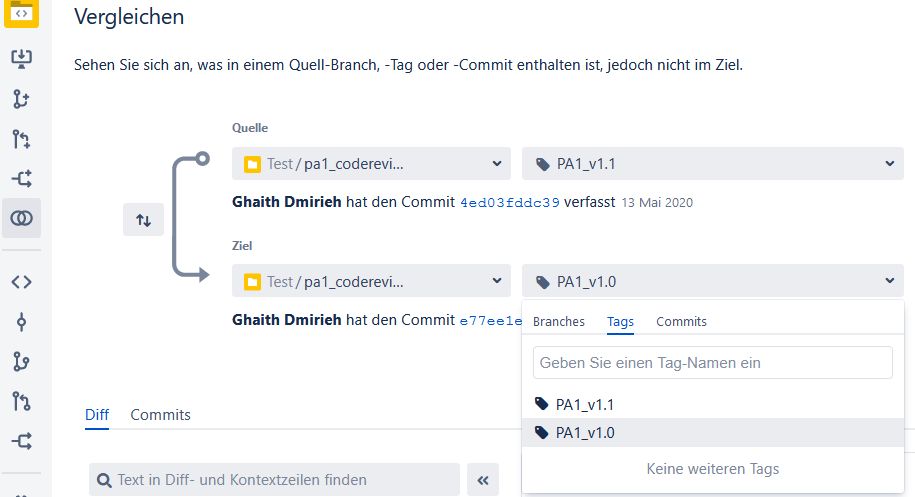
\includegraphics[width=1.0\textwidth]{BitbucketServerDiff}
	\caption[Flexibilität des Änderungsvergleichs auf Bitbucket-Server]{Flexibilität des Änderungsvergleichs \\Eigener Screenshot}
	\label{fig:Flexibilität des Änderungsvergleich}
\end{figure}

Die Änderungen können sowohl inline als auch side-by-side angezeigt werden. Ein Beispiel dafür ist die \cref{fig:BitbucketServerSideBySide}

\begin{figure}[H]
	\centering
	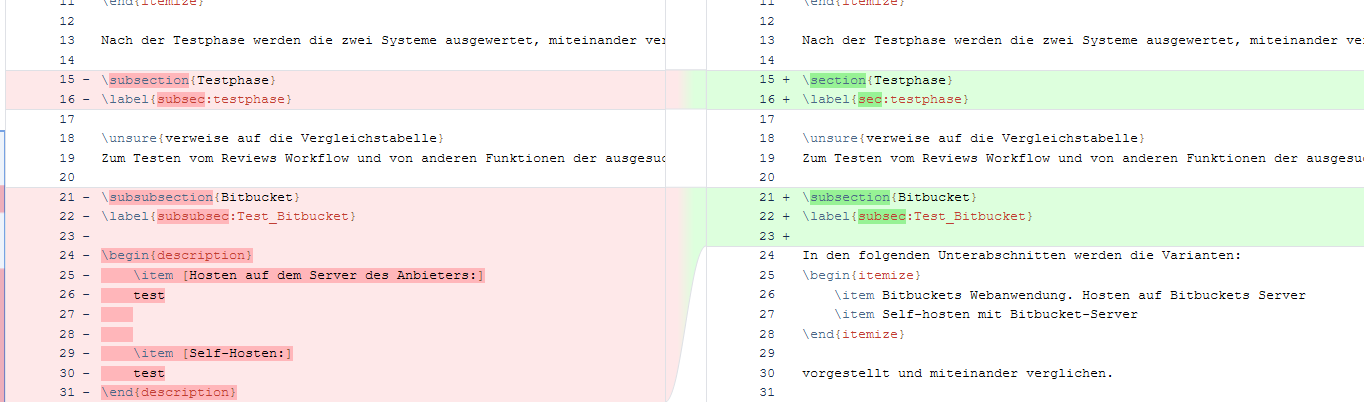
\includegraphics[width=1.0\textwidth]{BitbucketServerSideBySide}
	\caption[Side-by-side Änderungsvergleich auf Bitbucket-Server]{side-by-side Änderungsvergleich\\Eigener Screenshot}
	\label{fig:BitbucketServerSideBySide}
\end{figure}

Weil ein Pull-Request auf Bitbucket nur zwischen Branches möglich ist, sollen Features in abgespaltene Branches entwickelt und mit einem Pull Request zum Review abgesendet werden. Beim Erstellen eines Pull Requests werden zwei Branches markiert \footnote{Der Feature Branch, wo die Änderungen/Features entwickelt wurden und der Ziel-Branch, mit dem der Feature Branch zusammengeführt werden soll}. Die Nachrichten von jedem Commit auf dem Feature Branch werden in der Beschreibung des Pull Requests auftauchen, die auch editiert werden kann. Es ist auch möglich Dateien mit dem Pull Request zu schicken.
Der letzte Schritt ist das Hinzufügen von Reviewer, die die Änderungen überprüfen, kommentieren und dann annehmen oder ablehnen können. Die \cref{fig:BitbucketServer Pull-Request} verdeutlicht die erwähnten Schritte.

\begin{figure}[H]
	\centering
	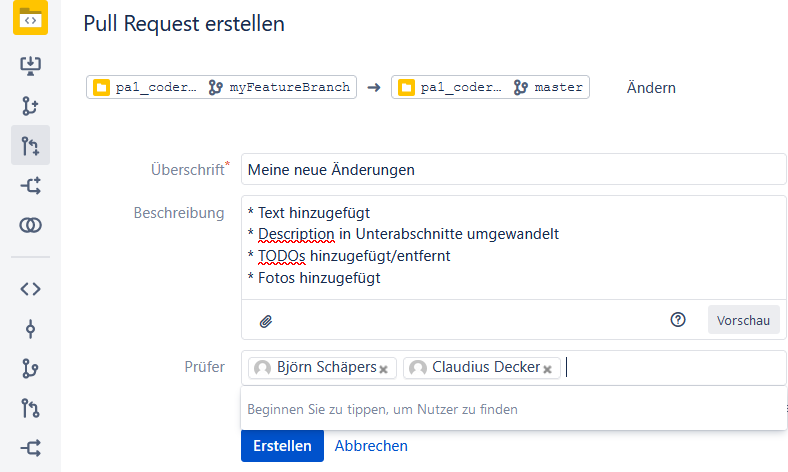
\includegraphics[width=1.0\textwidth]{BitbucketServer Pull-Request}
	\caption[Pull-Request auf Bitbucket-Server]{Pull-Request\\Eigener Screenshot}
	\label{fig:BitbucketServer Pull-Request}
\end{figure}

Die Reviewer haben diverse Möglichkeiten, wie sie auf bestimmte Teile eines Pull Requests reagieren. Diese Möglichkeiten sind:
\begin{itemize}
	\item Kommentare, auf sie auch vom Autor wieder kommentiert werden kann. Beispiel \cref{fig:BitbucketServerKommentar}.
	\begin{figure}[H]
		\centering
		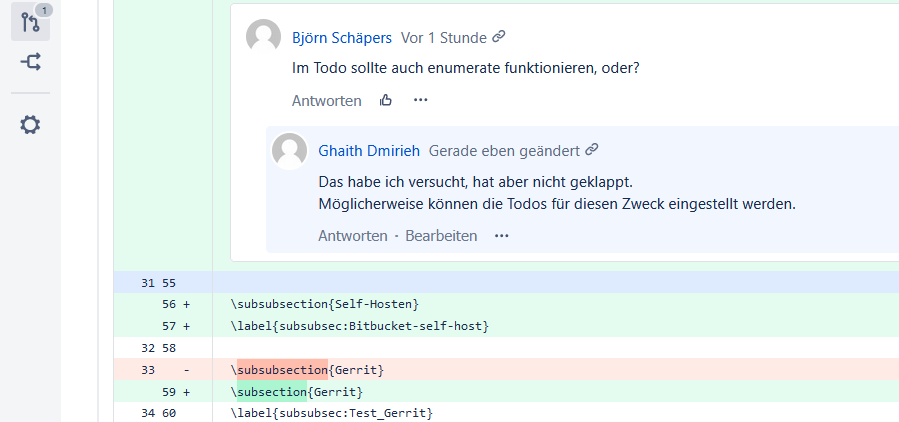
\includegraphics[width=1.0\textwidth]{BitbucketServerKommentar}
		\caption[Bitbucket-Server Kommentare]{Kommentare\\Eigener Screenshot}
		\label{fig:BitbucketServerKommentar}
	\end{figure}
	
	\item Direkte Änderungen im Quelltext machen, die der Autor als Vorschläge bekommt. Bei der Annahme dieser Vorschläge muss der Autor eine commit Nachricht schreiben, da diese 				Annahme als ein neues commit gesehen wird. Beispiel \cref{fig:BitbucketServer Vorschläge}.
	\begin{figure}[H]
		\centering
		\includegraphics[width=1.0\textwidth]{BitbucketServer Vorschläge}
		\caption[Bitbucket-Server Änderungsvorschläge]{Änderungsvorschläge\\Eigener Screenshot}
		\label{fig:BitbucketServer Vorschläge}
	\end{figure}
	
	
	\item Erstellen von Task-Liste. Reviewer können Aufgaben/Todos stellen, die vom Autor nach dem Einchecken der Bearbeitung dieser Aufgaben als erledigt markiert werden können. Beispiel 	\cref{fig:BitbucketServer Tasklist}.
	\begin{figure}[H]
		\centering
		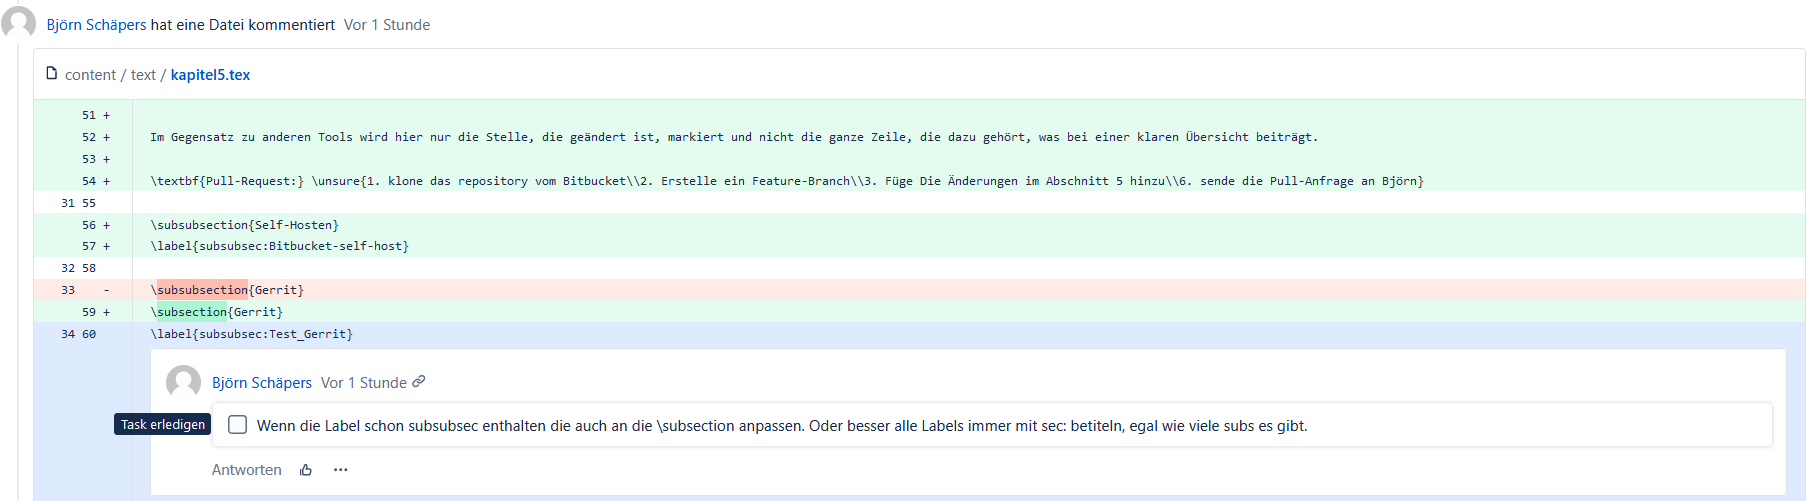
\includegraphics[width=1.0\textwidth]{BitbucketServer Tasklist}
		\caption[Bitbucket-Server Todos]{Todos/Aufgaben\\Eigener Screenshot}
		\label{fig:BitbucketServer Tasklist}
	\end{figure}
\end{itemize}

Bitbucket-Server bietet die volle Kontrolle auf das Pul Request, sodass das Team den Workflow der Arbeit an seine Bedürfnisse anpassen kann. Ein Pull Request von einem Feature Branch kann beispielsweise nur dann mit dem Ziel-Branch zusammengeführt werden, wenn alle Reviewer oder gewählte Reviewer das Pull Request bestätigen. Eine andere Möglichkeit wäre es, dass keine offenen Aufgaben dabei sind, wenn es gemergt werden soll. Diese Einstellung sind auf \cref{fig:BitbucketServer Merge-Checks} zu sehen.
\begin{figure}[H]
	\centering
	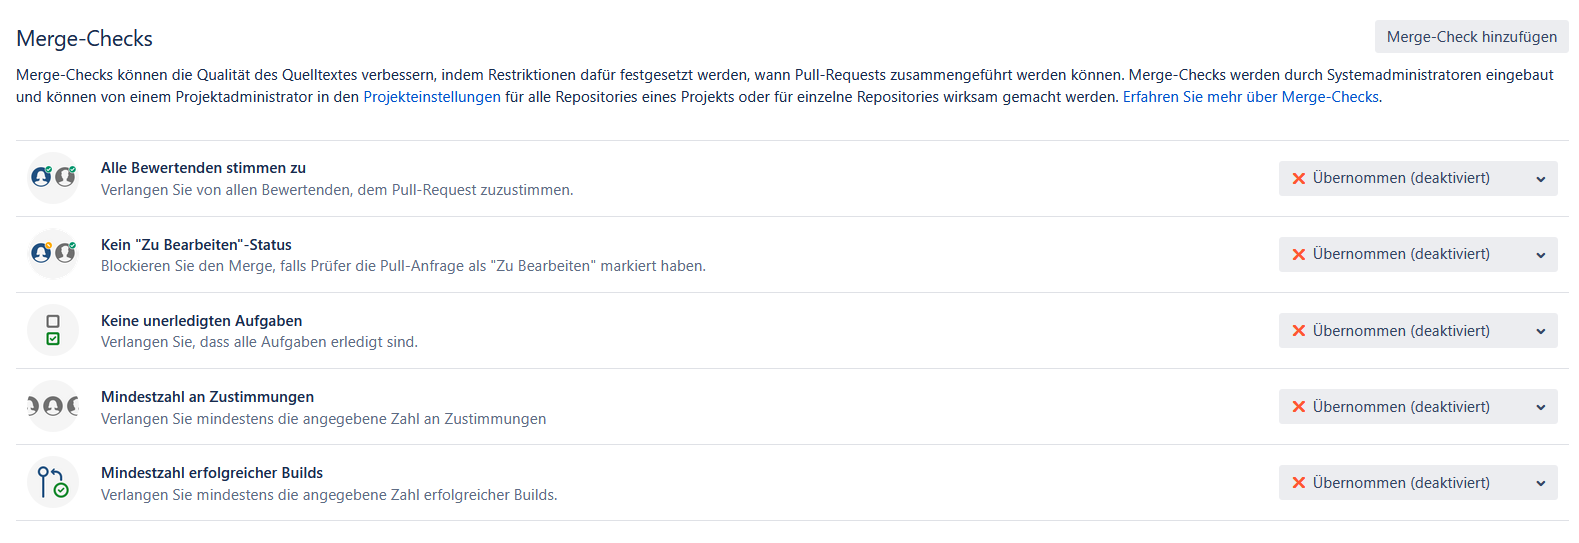
\includegraphics[width=1.0\textwidth]{Merge-Checks}
	\caption[BitbucketServer Merge-Checks]{BitbucketServer Merge-Checks\\Eigener Screenshot}
	\label{fig:BitbucketServer Merge-Checks}
\end{figure}

Außerdem kann der Administrator eines Projekts Beschränkungen auf die Commits einrichten z.B., dass nur bestimmte Benutzer in einem Repository ihre Änderungen einchecken können. Die \cref{fig:BitbucketServer Commits-Kontrolle} zeigt die mögliche Beschränkungen.

\begin{figure}[H]
	\centering
	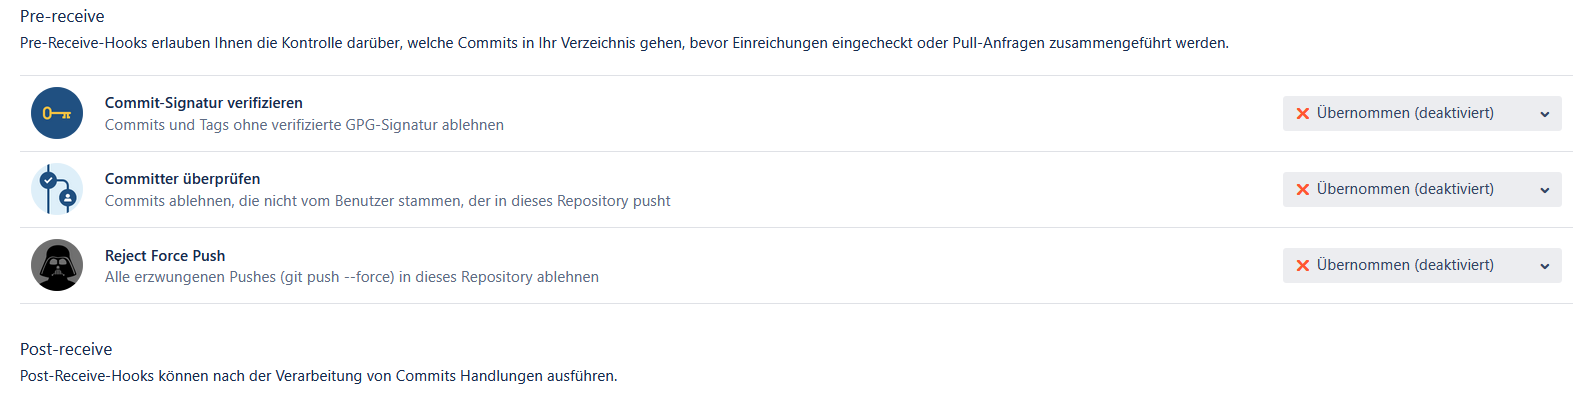
\includegraphics[width=1.0\textwidth]{Commits-Kontrolle}
	\caption[BitbucketServer Commits-Beschränkungen]{BitbucketServer Commits-Beschränkungen\\Eigener Screenshot}
	\label{fig:BitbucketServer Commits-Kontrolle}
\end{figure}

Nach dem die Reviewer sich das Pull Request angeschaut,Kommentiert und Aufgaben sowie Vorschläge gestellt haben und der Autor diese bearbeitet hat, wurde das Feature Branch mit dem Ziel-Branch zusammengeführt.

\subsection{Gerrit}
\label{subsubsec:Test_Gerrit}

Gerrit unterscheidet sich von den anderen Quellcodeverwaltungssysteme, da Gerrit mehr Gewicht auf das Review legt. Das System arbeitet ausschließlich mit dem \ac{VCS} Git und hat keine Cloud Version. D.h. bei Gerrit handelt es sich nur um self hosten. Die Installation auf odin erfolgte durch ein \textit{.war} Datei, die mit dem Befehl

{\color{blue}
\begin{verbatim}
	java -jar gerrit.war init -d <Pfad zur .war Datei> 
\end{verbatim}}

\noindent initialisieren lässt. Nach der Initialisierung müssen noch wichtige Konfigurationen in der datei \textit{gerrit.config}, die im Verzeichnis \textit{gerrit-Verzeichnis/etc} zu finden sind, eingestellt werden. Wie beispielsweise die Authentifizierung oder auch, wo Gerrit seine Projekte und Repositories anlegt. Das Programm kann danach mit dem Befehl

{\color{blue} 
\begin{verbatim}
	gerrit.sh start
\end{verbatim}}

\noindent gestartet werden. Diese Datei befindet sich im Verzeichnis \textit{Gerrit-Verzeichnis/bin}. Gerrit ist ab jetzt lauffähig und Projekte können erstellt werden. Um ein Projekt zu erstellen gibt es verschiedene Methoden. Hier wird ein Projekt via SSH erstellt, was durch den Befehl

{\color{blue}
\begin{verbatim}
	ssh -p <port> <host> gerrit create-project <Name des Projekts>
\end{verbatim}}

\noindent erfolgen lässt. Gerrit kann einfach als ein neues Remote für ein bestehendes Repository hinzugefügt werden. Schließlich werden die Commits dieses Repositorys mit dem Befehl

{\color{blue}
\begin{verbatim}
	git push <remote name> <host>/<project name>
\end{verbatim}}

\noindent auf Gerrit hochgeladen.

\subsubsection{Reviews Workflow}
\label{subsubsec:Reviews Workflow bei Gerrit}

Der erster Schritt ist das Hinzufügen ein \textbf{Change-Id} für die Commits. Dieses ID erlaubt Gerrit, verschiedene Versionen derselben Änderungen, die überprüft werden sollen, miteinander zu verknüpfen. Dieser Schritt ist durch die zwei Befehle

{\color{blue}
\begin{verbatim}
	scp -p -P <port> <host>:hooks/commit-msg <Pfad zum Repository>/.git/hooks/
	chmod u+x .git/hooks/commit-msg
\end{verbatim}}

\noindent zu erreichen. Ab jetzt können Änderungen reviewt werden, indem man die Änderungen in den Branch \textit{HEAD:refs/for/master} von gerrit pusht. Beispiel für die Review-Webseite auf Gerrit stellt die \cref{fig:Gerrit-Review} vor.

\begin{figure}[H]
	\centering
	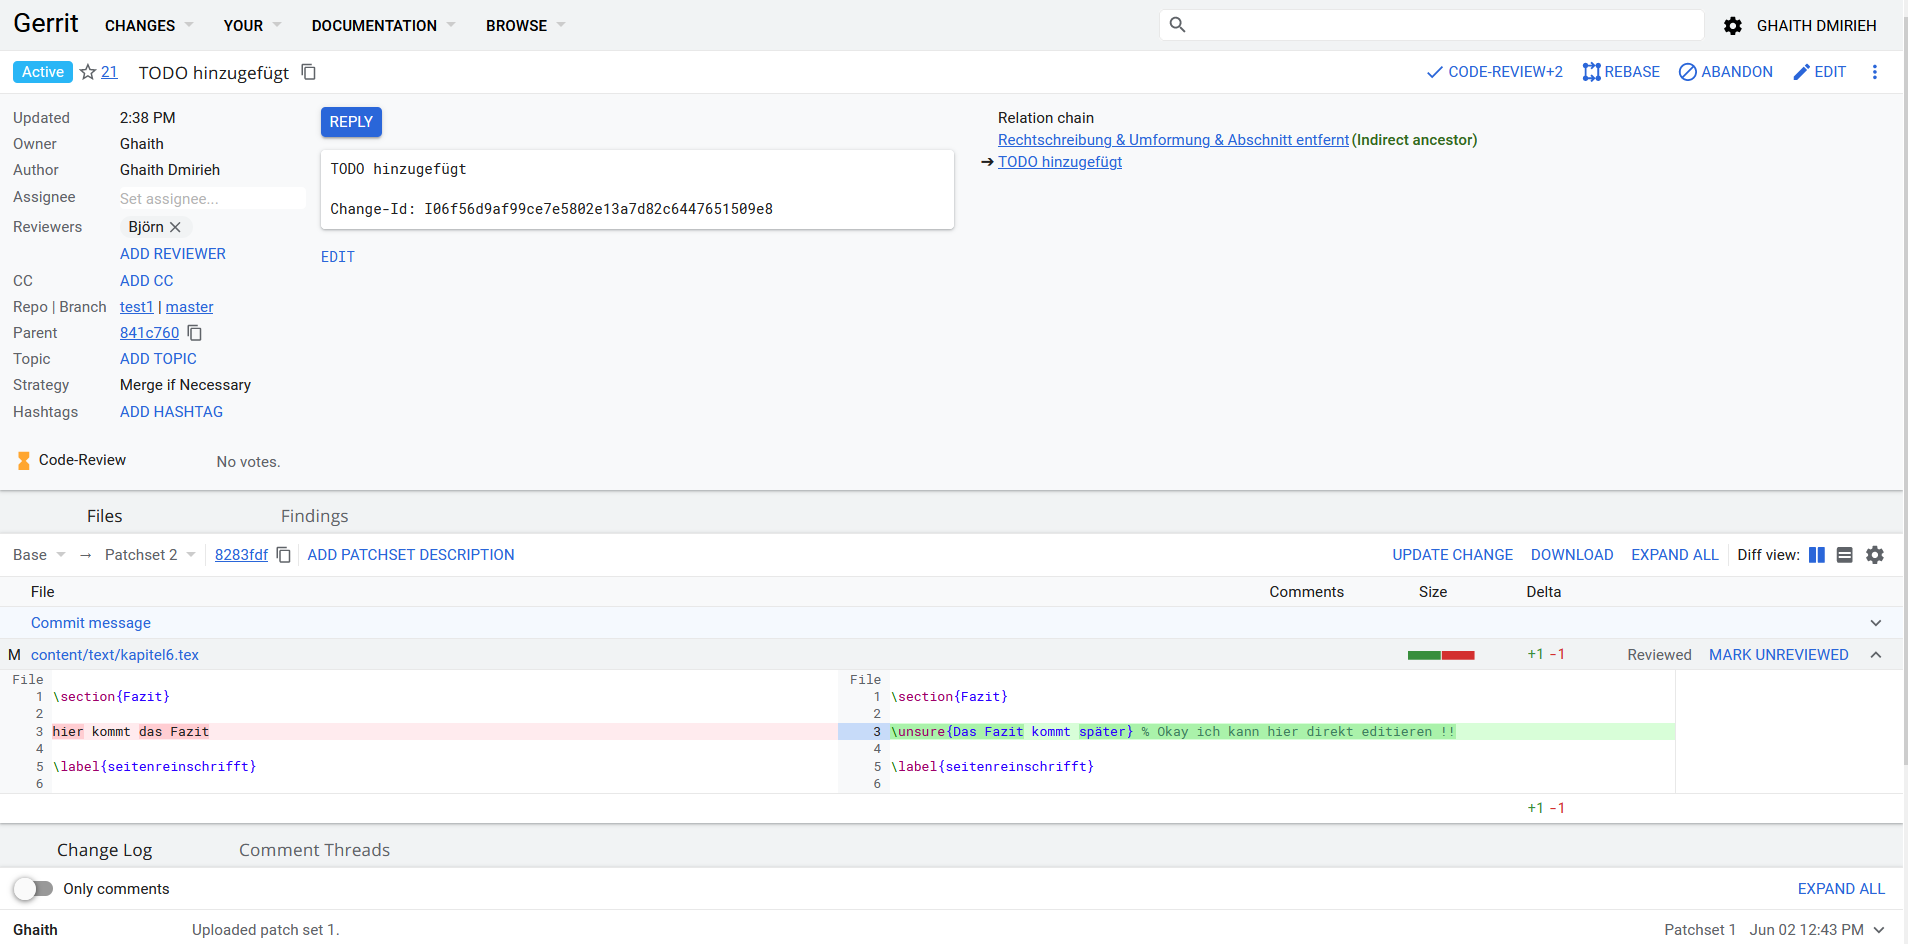
\includegraphics[width=1.0\textwidth]{Gerrit-Review}
	\caption[Gerrit Reviews Oberfläche]{Gerrit-Reviews Oberfläche\\Eigener Screenshot}
	\label{fig:Gerrit-Review}
\end{figure}

Auf dieser Webseite können die Reviewer hinzugefügt werden, die eine E-Mail bekommen, dass sie zum Review eingeladen sind. Gerrit verschickt auch E-Mails an den Autor Änderungen oder Kommentare vom Reviewer. Ebenfalls bekommen wieder die Reviewer E-Mails, wenn der Autor auf ihre Kommentare reagiert.

Reviewer haben die Möglichkeit auf Zeilenebene die Änderungen zu kommentieren. Beispiel dafür zeigt die \cref{fig:Gerrit Reviewer-Kommentare} 

\begin{figure}[H]
	\centering
	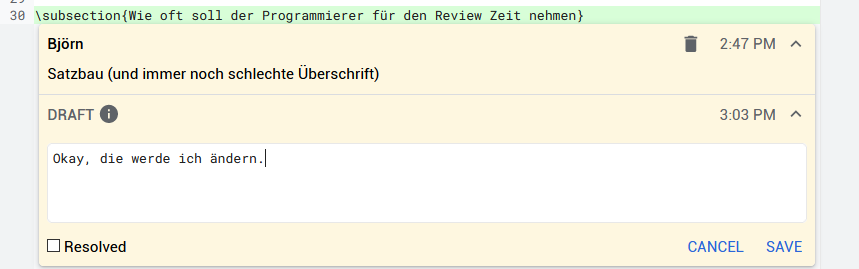
\includegraphics[width=1.0\textwidth]{Gerrit-Kommentar}
	\caption[Gerrit Reviewer-Kommentare]{Gerrit Reviewer-Kommentare\\Eigener Screenshot}
	\label{fig:Gerrit Reviewer-Kommentare}
\end{figure}

Was auch Gerrit ermöglicht, sind die direkte Änderungen am Quelltext. Reviewer sind imstande, ihre Meinung direkt am Quelltext zu äußern. Der Autor kann dann mithilfe von Git diese Vorschläge von den Reviewern übernehmen. Der Prozess erfolgt durch das Edit-Modus in der Webseite von Gerrit. Die \cref{fig:Gerrit Edit-Modus} zeigt dieses Modus.

\begin{figure}[H]
	\centering
	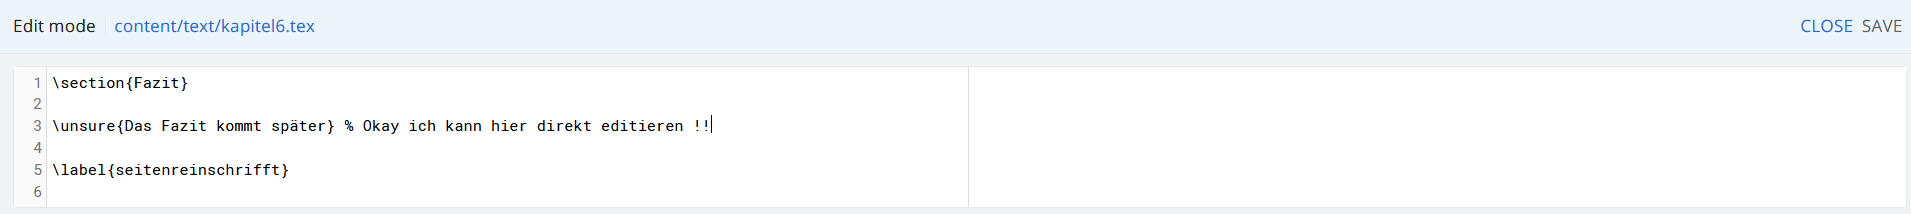
\includegraphics[width=1.0\textwidth]{Gerrit Edit}
	\caption[Gerrit Edit-Modus]{Gerrit Edit-Modus\\Eigener Screenshot}
	\label{fig:Gerrit Edit-Modus}
\end{figure}

Selber auf die Nachricht des Commits Können die Reviewer kommentieren. Beispiel dafür ist die \cref{fig:Gerrit Kommentar auf Commits Nachricht}

\begin{figure}[H]
	\centering
	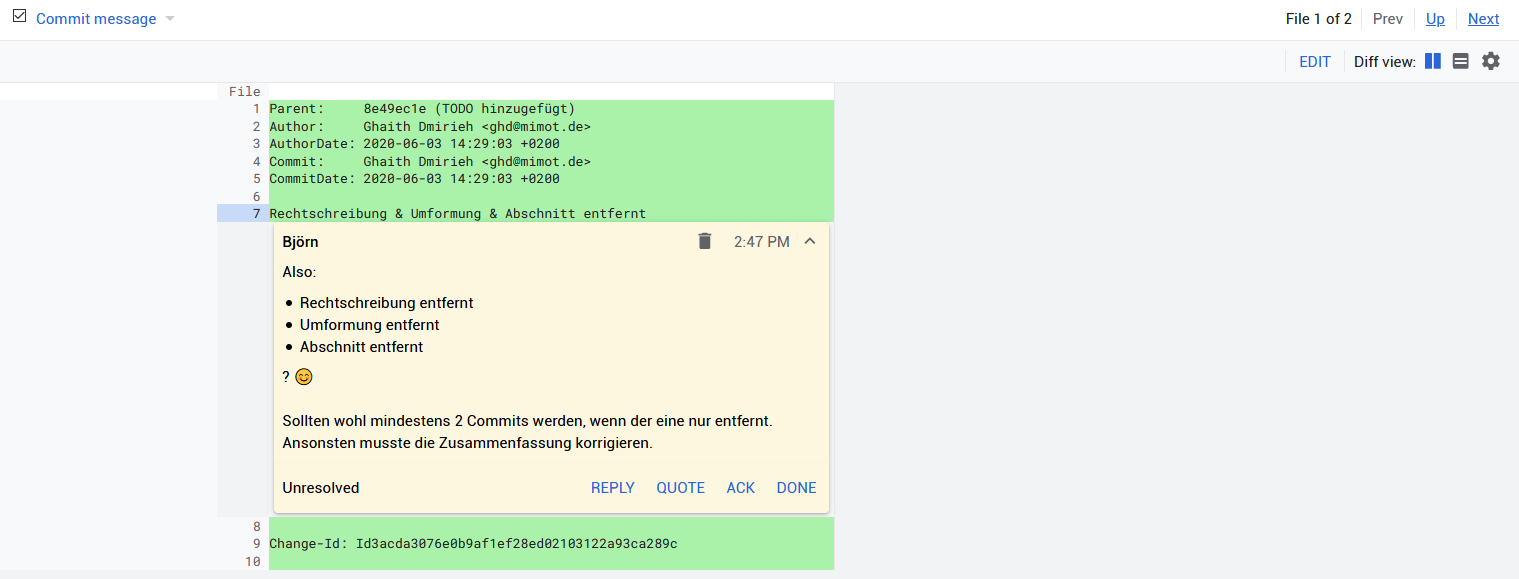
\includegraphics[width=1.0\textwidth]{Gerrit Kommentar auf Commits Nachricht}
	\caption[Gerrit Kommentar auf die Nachricht des Commits]{Gerrit Kommentar auf die Nachricht des Commits\\Eigener Screenshot}
	\label{fig:Gerrit Kommentar auf Commits Nachricht}
\end{figure}

Nachdem die Reviewer die Änderungen anschauen und darauf reagieren und ihre Vorschläge machen, bekommen die Antworten vom Autor, diese sind Kommentare oder Bearbeitung der Änderungen. Falls die Reviewer die bearbeitete Änderungen gut finden, können sie diese bestätigen. Erst wenn die Änderungen bestätigt sind, kann das Commit mit dem Ziel-Branch zusammengeführt werden.

Die Reviewer können auf 5 Ebenen die Änderungen bewerten, diese sind
\begin{compactitem}
	\item \textbf{-2} Abgelehnt, Die Änderungen dürfen nicht gemergt werden.
	\item \textbf{-1} Ich bestätige sie nicht. Die Änderungen müssen bearbeitet werden.
	\item \textbf{0}  Keine Punktzahl.
	\item \textbf{+1} Sieht für mich gut aus, aber jemand anderes muss sie noch bestätigen.
	\item \textbf{+2} Sieht gut aus. Ich bestätige sie.
\end{compactitem}

\subsection{Vergleich}
\label{subsec:Vergleich_Bitbucket_Gerrit}

Die zwei Systeme unterscheiden sich in zahlreichen Punkten, jedoch werden hier nicht alle in der Vergleichstabelle erscheinen, sondern nur die für die Abteilung wichtig sind. Diese Punkte verdeutlicht die \cref{table:Vergleichstabelle Gerrit & Bitbucket}

\begin{table}[h]
	\caption[Vergleichstabelle der ausgesuchten Systeme]{Vergleich der ausgesuchten Systeme}
	\centering
	\begin{tabular}{|c||c|c|}
			\hline 
			Eigenschaft & \textbf{Gerrit} & \textbf{Bitbucket Server} \\ 
			\hline 
			\textbf{\color{blue}{Review Workflow}} & Gerrit Branch & Pull Request \\ 
			\hline 
			\textbf{\color{blue}{Inline Diffs}} & \color{green}{\ja} & \color{green}{\ja} \\ 
			\hline 
			\textbf{\color{blue}{side by side Diffs}} & \color{green}{\ja} & \color{green}{\ja} \\ 
			\hline 
			\textbf{\color{blue}{Zugriffskontrolle auf Repo.}} & \color{green}{\ja} & \color{green}{\ja} \\ 
			\hline 
			\textbf{\color{blue}{Zugriffskontrolle auf den Reviews}} & \color{green}{\ja} & \color{green}{\ja} \\ 
			\hline 
			\textbf{\color{blue}{Vorschläge annehmen}} & \color{green}{\ja} & \color{green}{\ja} \\ 
			\hline 
			\textbf{\color{blue}{Patchsets}} & \color{green}{\ja} & \color{red}{\nein} \\ 
			\hline 
			\textbf{\color{blue}{E-Mail Benachrichtigungen}} & \color{green}{\ja} & \color{green}{\ja} \\ 
			\hline 
			\textbf{\color{blue}{Task-Liste}} & \color{red}{\nein} & \color{green}{\ja} \\
			\hline 
			\textbf{\color{blue}{Direkt Forken}} & \color{red}{\nein} & \color{green}{\ja} \\
			\hline 
			\textbf{\color{blue}{Diffs zwischen Commits/Tags/Branchs}} & \color{red}{\nein} & \color{green}{\ja} \\
			\hline 
			\textbf{\color{blue}{Kosten}} & Kostenfrei & Einmalige Zahlung \\
			\hline 
	\end{tabular} 
	\label{table:Vergleichstabelle Gerrit & Bitbucket}
\end{table}

\subsection{Auswertung}
\label{subsec:Auswertung}

Ganz wichtig zu erwähnen, dass um ein Pull Request zu erstellen, sollen die vom Pull Request betroffene Änderungen bereits in einem abgespaltenen Branch auf dem Remote-Repository stehen. D.h. Pull Requests sind mit Branchs engverbunden, was bestimmte Workflows erzwingt, demzufolge verringert dieser Prozess die Flexibilität vom \ac{VCS} Git, das die Entwickler ermöglicht, den Workflow an die Bedürfnisse des Teams anzupassen. Außerdem sind beispielsweise kleine Änderungen wie einen Fehler der korrigiert werden muss und seine Korrektur aus einer Zeile besteht, die jemanden anderen zuerst anschauen soll, nicht mehr flexibel, da dafür brauchen die Entwickler bei Bitbucket ein Branch zu erstellen. Im Gegensatz zu Gerrit kann man direkt im Haupt-Branch was ändern und ein Review dafür starten.

Bitbucket erleichtert die Arbeit mit seinen Funktionen in seiner Webseite, da man imstande ist, Branchs direkt in der Webseite zu erstellen oder sie abzuspalten. Im Gegensatz dazu hat Gerrit diese Funktionen nicht, da bei Gerrit es hauptsächlich um das Review geht. Beide Systeme können Zugriffsregeln auf die Repositories, Branchs oder auch wer reviewen darf erstellen, so dass nur bestimmte Entwickler daran arbeiten können.

Die Abteilung hat sich aus den folgenden Gründen

\begin{itemize}
	\item Bei Gerrit kann das Review unabhängig von dem Branch, an dem der Entwickler arbeitet, gestartet werden.
	\item Ist der Entwickler mit seinen Änderungen fertig und will sie in das Haupt-Branch einchecken und inzwischen hat jemand an das Haupt-Branch was geändert, dann kann Gerrit 		mit damit umgehen.
	\item Gerrit ist völlig kostenlos.
\end{itemize}

für Gerrit entschieden.
%-----------------------------------------------------------

\pagenumbering{Roman}
\setcounter{page}{\value{seitenanzahl}}
\pagestyle{plain.scrheadings}

\nocite{mcintosh2016empirical}

\nocite{mcintosh2014impact}

\nocite{Bjoern}

\nocite{HelixTeamHub}

\nocite{RhodeCode}

\nocite{Github}


\addsec{Quellenverzeichnis}
\printbibliography [heading=none]
\addsec{Anhang}
\appendix


\end{document}
